\documentclass[11pt,openany]{article}

\usepackage{mathtools, commath}
% Packages for formatting
\usepackage[margin=1in]{geometry}
\usepackage{fancyhdr}
\usepackage{enumerate}
\usepackage{graphicx}
\usepackage{kotex}
\usepackage{amsmath}
\usepackage{amsthm}
\usepackage[dvipsnames,table]{xcolor}
\usepackage{amssymb, amsfonts}

\usepackage{arydshln} % Include this package
% Fonts
\usepackage[T1]{fontenc}
\usepackage[utf8]{inputenc}
\usepackage{newpxtext,newpxmath}
\usepackage{sectsty}

% Define colors
\definecolor{TealBlue1}{HTML}{0077c2}
\definecolor{TealBlue2}{HTML}{00a5e6}
\definecolor{TealBlue3}{HTML}{b3e0ff}
\definecolor{TealBlue4}{HTML}{00293c}
\definecolor{TealBlue5}{HTML}{e6f7ff}

\definecolor{thmcolor}{RGB}{231, 76, 60}
\definecolor{defcolor}{RGB}{52, 152, 219}
\definecolor{lemcolor}{RGB}{155, 89, 182}
\definecolor{corcolor}{RGB}{46, 204, 113}
\definecolor{procolor}{RGB}{241, 196, 15}

\usepackage{color,soul}
\usepackage{soul}
\newcommand{\mathcolorbox}[2]{\colorbox{#1}{$\displaystyle #2$}}
\usepackage{cancel}
\newcommand\crossout[3][black]{\renewcommand\CancelColor{\color{#1}}\cancelto{#2}{#3}}
\newcommand\ncrossout[2][black]{\renewcommand\CancelColor{\color{#1}}\cancel{#2}}

\usepackage{hyperref}
\usepackage{booktabs}

% Chapter formatting
\definecolor{titleTealBlue}{RGB}{0,53,128}
\usepackage{titlesec}
\titleformat{\section}
{\normalfont\sffamily\Large\bfseries\color{titleTealBlue!100!gray}}{\thesection}{1em}{}
\titleformat{\subsection}
{\normalfont\sffamily\large\bfseries\color{titleTealBlue!50!gray}}{\thesubsection}{1em}{}

%Tcolorbox
\usepackage[most]{tcolorbox}
\usepackage{multirow}
\usepackage{multicol}

%Tikzpicture
\usepackage{tikz-cd}
\usetikzlibrary{positioning}
\usetikzlibrary{angles, quotes}
\usetikzlibrary{patterns,patterns.meta}

\usepackage[linesnumbered,ruled]{algorithm2e}
\usepackage{algpseudocode}
\usepackage{setspace}
\SetKwComment{Comment}{/* }{ */}
\SetKwProg{Fn}{Function}{:}{end}
\SetKw{End}{end}
\SetKw{DownTo}{downto}

% Define a new environment for algorithms without line numbers
\newenvironment{algorithm2}[1][]{
	% Save the current state of the algorithm counter
	\newcounter{tempCounter}
	\setcounter{tempCounter}{\value{algocf}}
	% redefine the algorithm numbering (remove prefix)
	\renewcommand{\thealgocf}{}
	\begin{algorithm}
	}{
	\end{algorithm}
	% Restore the algorithm counter state
	\setcounter{algocf}{\value{tempCounter}}
}

\usepackage{adjustbox}
% Header and footer formatting
\pagestyle{fancy}
\fancyhead{}
\fancyhf{}
\rhead{Student ID: \textbf{F2025014}\quad Name: \textbf{지용현}}%\rule{3cm}{0.4pt}}
\lhead{\textcolor{TealBlue2}{\textbf{[2025 Fall] Complex Analysis}}}
% Define footer
\newcommand{\footer}[1]{
\begin{flushright}
	\vspace{2em}
	\includegraphics[width=3cm]{school_logo.jpg} \\
	\vspace{1em}
	\textcolor{TealBlue2}{\large\textbf{#1}}
\end{flushright}
}
%\rfoot{\large Department of Information Security, Cryptogrphy and Mathematics, Kookmin Uni.\includegraphics[height=1.5cm]{school_logo.jpg}}
\fancyfoot{}
\fancyfoot[C]{-\thepage-}

\newcommand{\ie}{\textnormal{i.e.}}
\newcommand{\rsa}{\mathsf{RSA}}
\newcommand{\rsacrt}{\mathsf{RSA}\textendash\mathsf{CRT}}
\newcommand{\inv}[1]{#1^{-1}}

\usepackage{amsthm}
\newtheorem{axiom}{Axiom}[section]
\newtheorem{theorem}{Theorem}
\newtheorem*{theorem*}{Theorem}
\newtheorem{proposition}[theorem]{Proposition}
\newtheorem{corollary}{Corollary}[theorem]
\newtheorem*{corollary*}{Corollary}
\newtheorem{lemma}[theorem]{Lemma}
\newtheorem*{lemma*}{Lemma}

\theoremstyle{definition}
\newtheorem{definition}{Definition}
\newtheorem*{definition*}{Definition}
\newtheorem*{note}{Note}
\newtheorem{remark}{Remark}
\newtheorem{example}{Example}
\newtheorem{exercise}{Exercise}[section]

%New Command
%\newcommand{\set}[1]{\left\{#1\right\}}
\newcommand{\N}{\mathbb{N}}
\newcommand{\Z}{\mathbb{Z}}
\newcommand{\Q}{\mathbb{Q}}
\newcommand{\R}{\mathbb{R}}
\newcommand{\C}{\mathbb{C}}
\newcommand{\F}{\mathbb{F}}
\newcommand{\nbhd}{\mathcal{N}}
\newcommand{\Log}{\operatorname{Log}}
\newcommand{\Arg}{\operatorname{Arg}}
\newcommand{\pv}{\operatorname{P.V.}}

\newcommand{\of}[1]{\left( #1 \right)} 
%\newcommand{\abs}[1]{\left\lvert #1 \right\rvert}
%\newcommand{\norm}[1]{\left\| #1 \right\|}

\newcommand{\sol}{\textcolor{magenta}{\bf Sol}}
\newcommand{\conjugate}[1]{\overline{#1}}

\newcommand{\res}{\operatorname{res}}
\DeclareMathOperator*{\Res}{\operatorname{Res}}

\renewcommand{\Re}{\operatorname{Re}}
\renewcommand{\Im}{\operatorname{Im}}

\newcommand{\cyclic}[1]{\langle #1 \rangle}
\newcommand{\uniform}{\overset{\$}{\leftarrow}}

\newcommand{\Sol}{{\color{magenta}\normalfont\bfseries\text{Sol}}}
\renewcommand{\d}{\mathrm{d}} % For the exterior derivative 'd'


\tcbset{
%	colframe=myframecolor, % Set default frame color
	colback=white,    % Set default background color
	% You can add other default options here, e.g., arc=2mm, boxrule=0.5mm, etc.
}

\setstretch{1.25}
\begin{document}
\pagenumbering{arabic}
\begin{center}
	\Huge\textbf{Complex Analysis}\\
	\vspace{0.5em}
	\normalsize{\today}\\
%	\vspace{0.5em}
%	\large\quad\textbf{F2025014\qquad Ji, Yonghyeon}\\
	\vspace{0.5em}
\end{center}
\tableofcontents

\section{Complex numbers}
\begin{tcolorbox}
Verify that $\sqrt{2}\,|z|\ge |\Re z|+|\Im z|$.
\end{tcolorbox}
	\begin{proof}[\Sol]
	Let $z=x+iy$, so that $x=\Re z$, $y=\Im z$, and $\lvert z\rvert=\sqrt{x^2+y^2}$. Then
	\begin{align*}
		\sqrt{2}\,\lvert z\rvert \;\ge\; \lvert \Re z\rvert+\lvert \Im z\rvert&\iff\sqrt{2}\,\sqrt{x^2+y^2}\;\ge\;\lvert x\rvert+\lvert y\rvert\\
		&\iff 2(x^2+y^2)\;\ge\;(\lvert x\rvert+\lvert y\rvert)^2\\
		&\iff 2(x^2+y^2)\;\ge\;x^2+y^2+2\lvert x\rvert\lvert y\rvert\quad(\because |x|^2=x^2,\; |y|^2=y^2)\\
		&\iff x^2+y^2\;\ge\;2\lvert x\rvert\lvert y\rvert\quad\text{by subtracting $x^2+y^2$ from both sides}\\
		&\iff x^2+y^2\;\ge\;2\sqrt{x^2y^2} \\
		&\iff \frac{x^2+y^2}{2}\;\ge\;\sqrt{x^2y^2} \\
		&\iff \frac{a+b}{2}\;\ge\;\sqrt{ab}\quad\text{by setting $a:=x^2$ and $b:=y^2$;\quad (AM-GM inequality)} \\
	\end{align*}
	Hence it holds.
	\begin{center}
		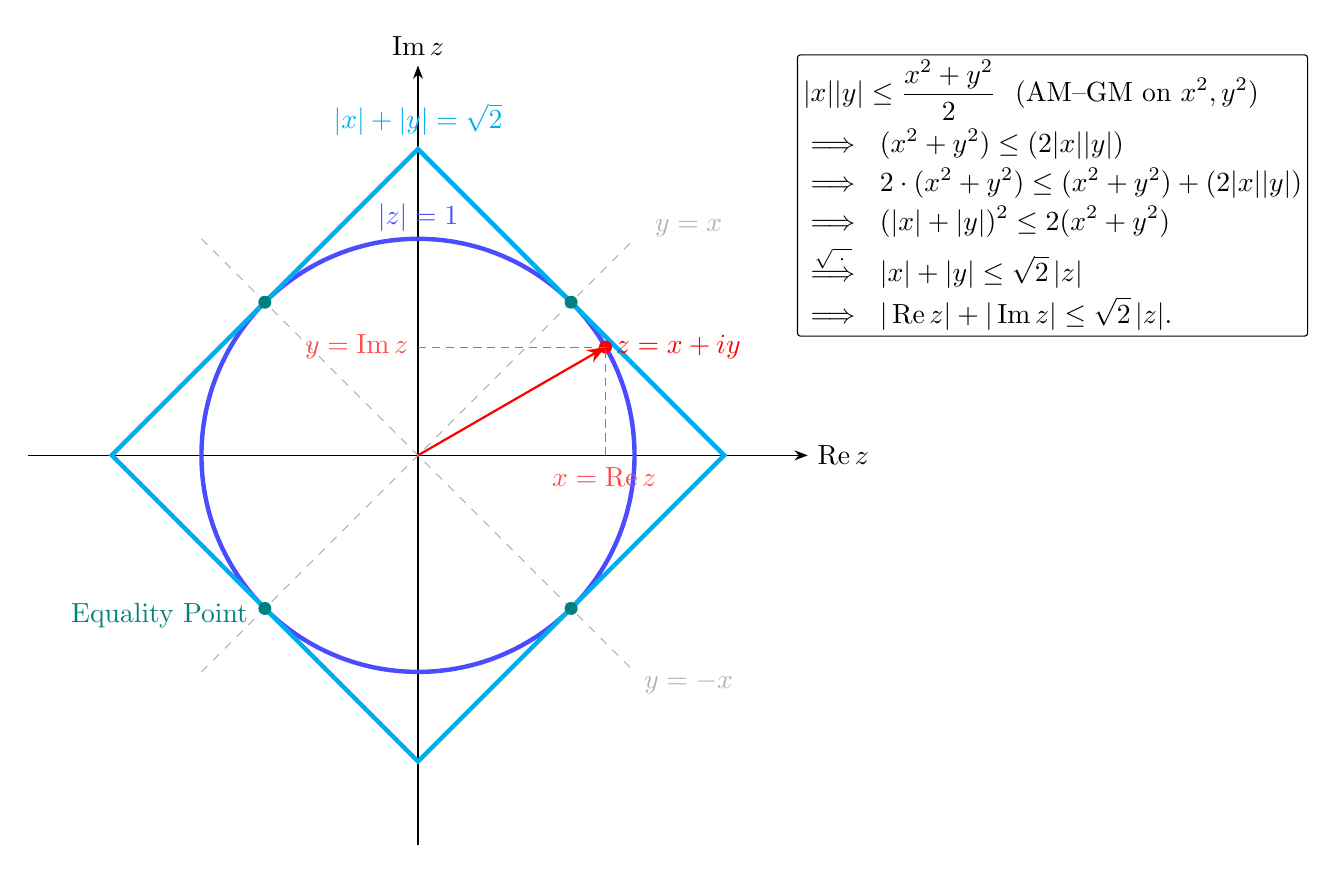
\begin{tikzpicture}[scale=2.75, >=Stealth]
			% axes
			\draw[->] (-1.8,0) -- (1.8,0) node[right] {$\Re z$};
			\draw[->] (0,-1.8) -- (0,1.8) node[above] {$\Im z$};
			
			% unit circle |z|=1
			\draw[ultra thick,blue!70] (0,0) circle (1);
			%	\draw[ultra thick,blue!70, opacity=.5] (0,0) circle (0.7207);
			\node[blue!70] at (0,1.1) {$|z|=1$};
			
			% diamond |x|+|y|=sqrt(2)  (vertices at (±√2,0),(0,±√2))
			% use √2 ≈ 1.4142
			\draw[ultra thick,cyan] ( 1.4142,0) -- (0, 1.4142) -- (-1.4142,0) -- (0,-1.4142) -- cycle;
			\node[cyan] at (0,1.55) {$|x|+|y|=\sqrt{2}$};
			
			% equality rays y=±x
			\draw[dashed,gray!60] (-1,-1) -- (1,1);
			\draw[dashed,gray!60] (-1, 1) -- (1,-1);
			\node[gray!60] at (1.25,1.05) {$y=x$};
			\node[gray!60] at (1.25,-1.05) {$y=-x$};
			
			\foreach \X/\Y in {0.7071/0.7071, 0.7071/-0.7071, -0.7071/0.7071, -0.7071/-0.7071}{
				\fill[teal] (\X,\Y) circle (0.03);
			}
			\node[teal,anchor=east] at (-0.74,-0.74) {Equality Point
				%		$\bigl(\tfrac{1}{\sqrt2},\tfrac{1}{\sqrt2}\bigr)$
			};
			
			% a sample point on the circle (theta = 30°)
			% coordinates: (cos 30°, sin 30°) ≈ (0.8660, 0.5)
			\fill[red] (0.8660,0.5000) circle (0.03);
			\draw[red,->,thick] (0,0) -- (0.8660,0.5000) node[right] {$z=x+iy$};
			
			% helper projections to visualize |x| and |y|
			\draw[red!70,densely dashed] (0.8660,0) -- (0.8660,0.5000);
			\draw[red!70,densely dashed] (0,0.5000) -- (0.8660,0.5000);
			\node[red!70] at (0.86,-0.10) {$x=\Re z$};
			\node[red!70, left] at (0,0.50) {$y=\Im z$};
			
			% AM-GM derivation (compact)
			\node[align=left,draw,rounded corners=1pt,inner sep=2pt,anchor=west] at (1.75,1.2)
			{$\displaystyle |x||y|\le\frac{x^2+y^2}{2}\ \ (\text{AM--GM on }x^2,y^2)$\\[2pt]
				$\displaystyle \implies\ (x^2+y^2)\le (2|x||y|)$\\[2pt]
				$\displaystyle \implies\ 2\cdot (x^2+y^2)\le(x^2+y^2)+(2|x||y|)$\\[2pt]
				$\displaystyle \implies\ (|x|+|y|)^2\le 2(x^2+y^2)$\\[2pt]
				$\displaystyle \overset{\sqrt{\;\cdot\;}}{\implies}\ |x|+|y|\le \sqrt{2}\,|z|$\\[2pt]
				$\displaystyle \implies\ |\Re z|+|\Im z|\le \sqrt{2}\,|z|.$};
		\end{tikzpicture}
	\end{center}
\end{proof}
\begin{tcolorbox}
By factoring $z^4-4z+3$ into two quadratic factors show that if $z$ lies on the circle $|z|=2$, then \[
\left|\frac{1}{z^4-4z^2+3}\right|\le \frac13.
\]
\end{tcolorbox}
\begin{proof}[\Sol]
	Since $z^4-4z^2+3 \;=\; (z^2-1)(z^2-3)$, we have \[
	\left\lvert z^4-4z^2+3 \right\rvert
	= \lvert z^2-1\rvert\,\lvert z^2-3\rvert.
	\]
	For $\lvert z\rvert=2$ one has $\lvert z^2\rvert=\lvert z\rvert^2=4$. By the triangle inequality,
	\[
	\lvert z^2-1\rvert \;\ge\; \bigl|\,\lvert z^2\rvert-\lvert 1\rvert\,\bigr| = \lvert 4-1\rvert = 3,
	\qquad
	\lvert z^2-3\rvert \;\ge\; \bigl|\,\lvert z^2\rvert-\lvert 3\rvert\,\bigr| = \lvert 4-3\rvert = 1.
	\]
	Hence
	\[
	\lvert z^4-4z^2+3\rvert \;\ge\; 3\cdot 1 \;=\; 3,
	\]
	and therefore
	\[
	\left\lvert\frac{1}{z^4-4z^2+3}\right\rvert \;=\; \frac{1}{\lvert z^4-4z^2+3\rvert} \;\le\; \frac{1}{3}.
	\]
	
	\begin{center}
		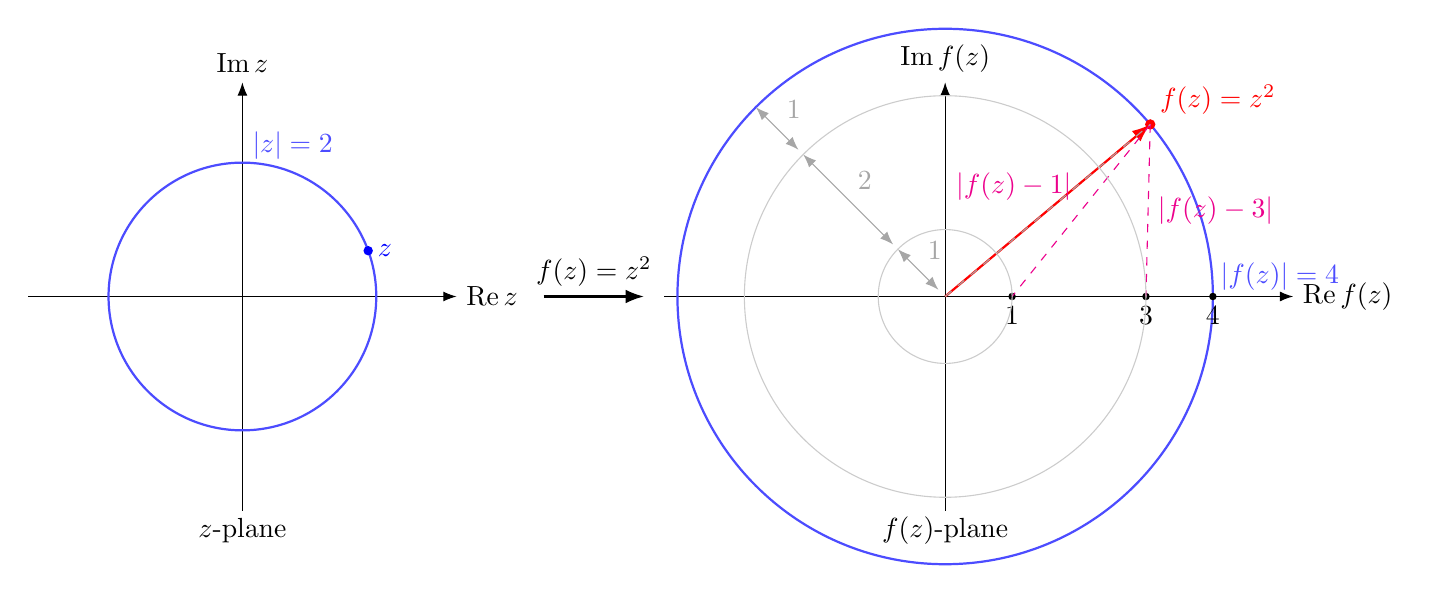
\begin{tikzpicture}[>=Latex,scale=.85]
			
			%================ z-plane =================
			\begin{scope}
				% axes
				\draw[->] (-3.2,0) -- (3.2,0) node[right] {$\Re z$};
				\draw[->] (0,-3.2) -- (0,3.2) node[above] {$\Im z$};
				\node at (0,-3.5) {$z$-plane};
				
				% circle |z|=2
				\draw[thick,blue!70] (0,0) circle (2);
				\node[blue!70] at (0.75,2.25) {$|z|=2$};
				
				% sample point z with |z|=2, angle ~20°
				% coordinates: 2*(cos20, sin20) ≈ (1.8794, 0.6840)
				\fill[blue] (1.8794,0.6840) circle (2pt)
				node[anchor=west] {$z$};
				
				% mapping arrow
				\draw[->,thick] (4.5,0) -- (6,0) node[midway,above] {$f(z)=z^2$};
			\end{scope}
			
			%================ w-plane =================
			\begin{scope}[xshift=10.5cm]
				% axes
				\draw[->] (-4.2,0) -- (5.2,0) node[right] {$\Re f(z)$};
				\draw[->] (0,-3.2) -- (0,3.2) node[above] {$\Im f(z)$};
				\node at (0,-3.5) {$f(z)$-plane};
				
				% circle |w|=4
				\draw[thick,blue!70] (0,0) circle (4);
				\node[blue!70] at (5,0.3) {$|f(z)|=4$};
				
				% two real points 1 and 3
				\fill (1,0) circle (1.6pt) node[below] {$1$};
				\fill (3,0) circle (1.6pt) node[below] {$3$};;
				\fill (4,0) circle (1.6pt) node[below] {$4$};
				
				% image point w = z^2 (angle doubles: ~40°), coords 4*(cos40, sin40) ≈ (3.0640, 2.5712)
				\fill[red] (3.0640,2.5712) circle (2.2pt) node[above right] {$f(z)=z^2$};
				\draw[red,->,thick] (0,0) -- (3.0640,2.5712);
				
				% distances |w-1| and |w-3|
				\draw[magenta, dashed] (3.0640,2.5712) -- (1,0) node[midway,above left] {$|f(z)-1|$};
				\draw[magenta, dashed] (3.0640,2.5712) -- (3,0) node[midway,right] {$|f(z)-3|$};
				
				% triangle-inequality lower bounds along the radial (origin->w) direction
				% show the radial segment length 4, and compare to 1 and 3
				\draw[dashed,gray!70] (0,0) -- (3.0640,2.5712); % radius 4
				% project the points 1 and 3 to the radial line via concentric circles
				\draw[gray!40] (0,0) circle (1);
				\draw[gray!40] (0,0) circle (3);
				
				% double-arrows indicating |4-1|=3 and |4-3|=1 on the radial line
				% place them near the ray with small offsets for clarity
				% marker for 0->1
				\draw[<->,gray!70] (-0.10,0.10) -- (-0.7071,0.7071)
				node[midway,above right] {$1$};
				% marker for 1->3
				\draw[<->,gray!70] (-0.7771,0.7771) -- (-2.1213,2.1213)
				node[midway,above right] {$2$};
				% marker for 3->4
				\draw[<->,gray!70] (-2.1913,2.1913) -- (-2.8284,2.8284)
				node[midway,above right] {$1$};
				%		% marker for 0->4 (whole radius)
				%		\node[gray!70] at (-1.9,1.2) {$|w|=4$};
				
				%		% inequality reminders near the base points
				%		\node[align=left,gray!60] at (0.9,1.3)
				%		{$|w-1| \ge \bigl||w|-1\bigr|=3$};
				%		\node[align=left,gray!60] at (2.6,-1.1)
				%		{$|w-3| \ge \bigl||w|-3\bigr|=1$};
				
				%		% product and reciprocal bounds
				%		\node[draw,rounded corners=2pt,align=left,anchor=west] at (-3.0,-2.4)
				%		{$\displaystyle |(w-1)(w-3)| \ge 3\cdot1=3$\\[4pt]
					%			$\displaystyle \left|\frac{1}{(w-1)(w-3)}\right| \le \frac{1}{3}$};
			\end{scope}
		\end{tikzpicture}
	\end{center}
\end{proof}
\begin{tcolorbox}
Prove that the usual formula solves the quadratic equation \[
az^2+bz+c=0\quad (a\neq 0)
\] when the coefficient $a$,$b$, and $c$ are complex numbers. Specifically, by completing the square on the left-hand side, derive the \textbf{quadratic formula} \[
z=\frac{-b+\sqrt{b^2-4ac}}{2a},
\] where both square roots are to be considered when $b^2-4ac\neq 0$. Use this result to find the roots of the equation \[
z^2+2z+(1-i)=0.
\]
\end{tcolorbox}
\begin{proof}[\Sol]
	Since  \[
	az^2+bz+c
	= a\!\left(z^2+\frac{b}{a}z\right)+c
	= a\!\left(z+\frac{b}{2a}\right)^{\!2}-a\!\left(\frac{b}{2a}\right)^{\!2}+c
	= a\!\left(z+\frac{b}{2a}\right)^{\!2}-\frac{b^2}{4a}+c,
	\] we have
	\[
	a\!\left(z+\frac{b}{2a}\right)^{\!2}=\frac{b^2}{4a}-c
	\quad\Longleftrightarrow\quad
	\left(z+\frac{b}{2a}\right)^{\!2}=\frac{b^2-4ac}{4a^2}.
	\]
	Taking square roots of both sides yields \[
	z+\frac{b}{2a}=\,\frac{\sqrt{\,b^2-4ac\,}}{2a},\quad\text{whence}\quad z=\frac{-b+\sqrt{\,b^2-4ac\,}}{2a}.
	\] Consider $z^2+2z+(1-i)$ with \(a=1\), \(b=2\), and \(c=1-i\). The discriminant is \[
	\Delta=b^2-4ac=4-4(1-i)=4i.
	\] Since \[
	\sqrt{i}=\frac{1+i}{\sqrt{2}}\quad\left(\text{indeed},\; \left(\frac{1+i}{\sqrt{2}}\right)^2=\frac{1+2i-1}{2}=i\right),
	\] we may take $\sqrt{\Delta}=\sqrt{4i}=2\sqrt{i}= \sqrt{2}\,(1+i)$.
	Therefore \[
	z=\frac{-2\pm \sqrt{4i}}{2}
	= -1 \pm \sqrt{i}
	= -1 \pm \frac{1+i}{\sqrt{2}}.
	\] Thus the roots are \[
	z_1=-1+\frac{1+i}{\sqrt{2}},
	\qquad
	z_2=-1-\frac{1+i}{\sqrt{2}}.
	\] Note that $z_1,z_2$ are roots of $(z+1)^2=i$.
	
	\begin{center}
		\adjustbox{scale=.7,center}{
		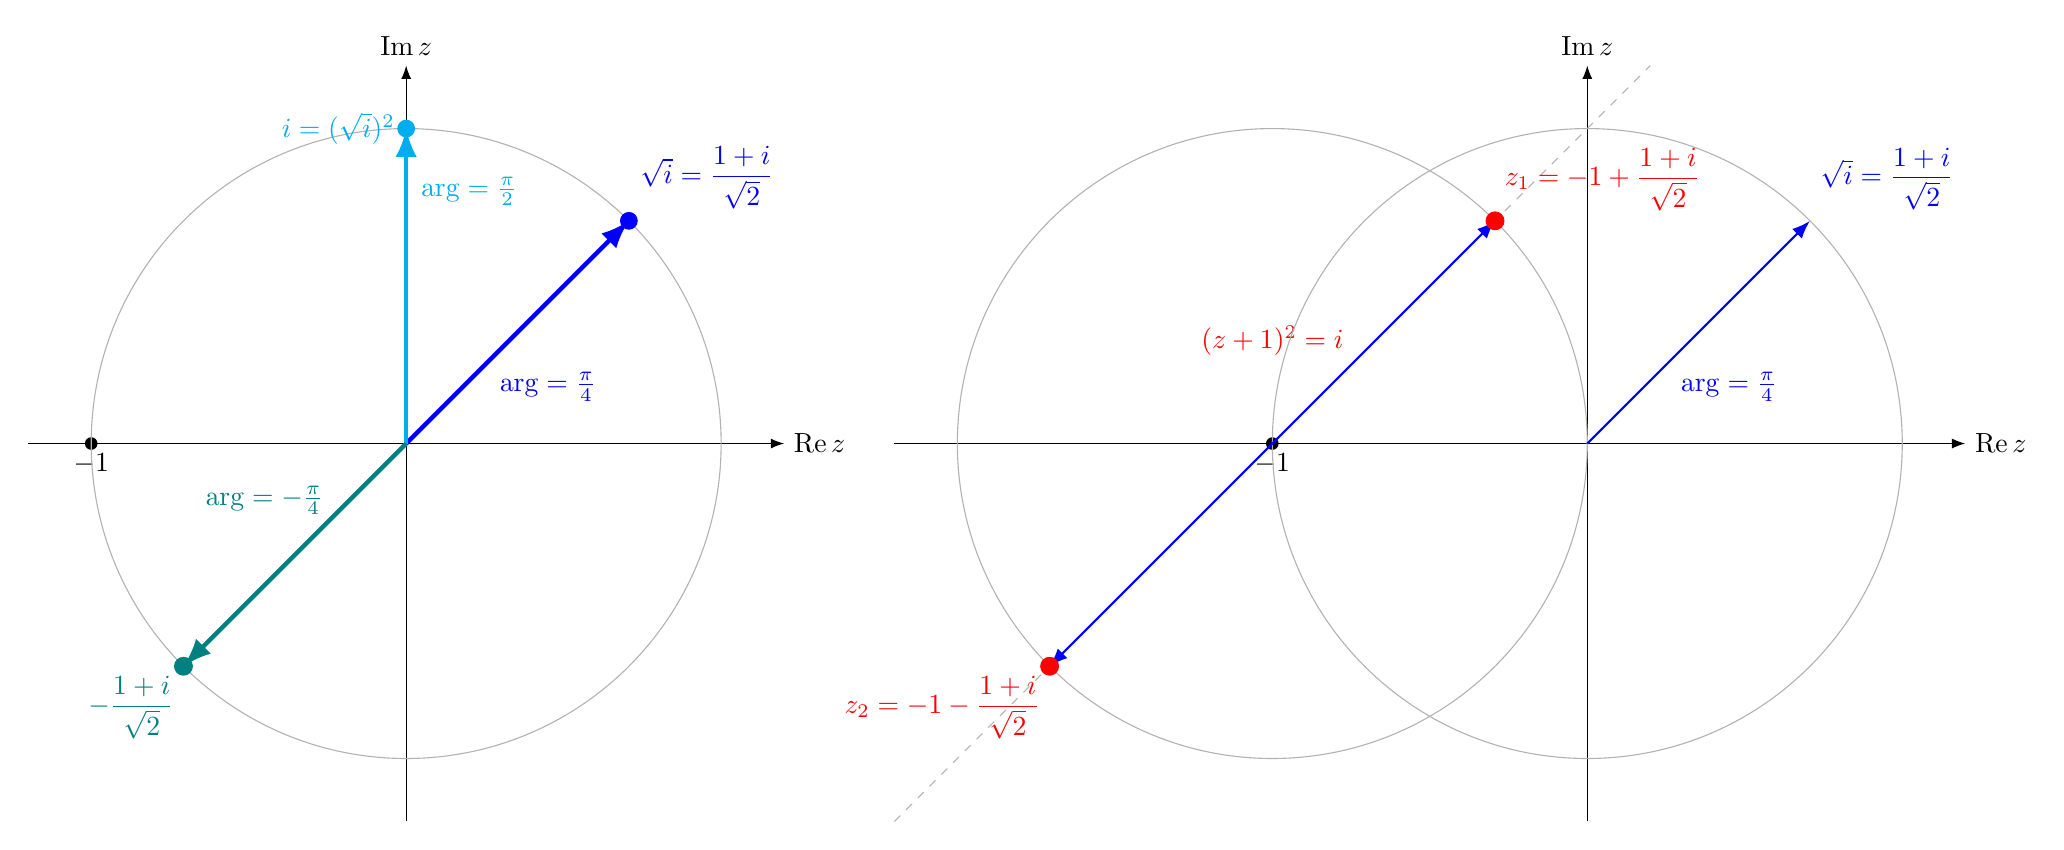
\begin{tikzpicture}[>=Latex, scale=4.0]
			% Axes
			\draw[->] (-1.2,0) -- (1.2,0) node[right] {$\Re z$};
			\draw[->] (0,-1.2) -- (0,1.2) node[above] {$\Im z$};
			% Center at -1 + 0i (from completing the square: (z+1)^2 = i)
			\fill (-1,0) circle (0.02) node[below] {$-1$};
			\draw[gray!60] (0,0) circle (1);
			\draw[blue,->, ultra thick] (0,0) -- (0.7071,0.7071)
			node[above right] {$\sqrt{i}=\dfrac{1+i}{\sqrt2}$};
			\filldraw[blue] (0.7071,0.7071) circle (.75pt);
			\node[blue] at (0.45,0.18) {$\arg=\tfrac{\pi}{4}$};
			\draw[cyan,->, ultra thick] (0,0) -- (0,1)
			node[left] {$i=(\sqrt{i})^2$};
			\filldraw[cyan] (0,1) circle (.75pt);
			\node[cyan] at (.2,0.8) {$\arg=\tfrac{\pi}{2}$};
			\draw[teal,->,ultra thick] (0,0) -- (-.7071,-.7071);
			% Roots as endpoints on the circle
			\fill[teal] (-.7071,-.7071) circle (0.03)
			node[below left] {$-\dfrac{1+i}{\sqrt2}$};
			\node[teal] at (-.45,-.18) {$\arg=-\tfrac{\pi}{4}$};
			\begin{scope}[xshift=3.75cm]
				% Axes
				\draw[->] (-2.2,0) -- (1.2,0) node[right] {$\Re z$};
				\draw[->] (0,-1.2) -- (0,1.2) node[above] {$\Im z$};
				% Center at -1 + 0i (from completing the square: (z+1)^2 = i)
				\node[above, red] at (-1,.25) {$(z+1)^2 = i$};
				\fill (-1,0) circle (0.02) node[below] {$-1$};
				% Guide: circle of radius 1/sqrt(2) centered at -1
				% 1/sqrt(2) ≈ 0.7071
				%\draw[gray!60] (-1,0) circle (0.7071);
				\draw[gray!60] (-1,0) circle (1);
				\draw[gray!60] (0,0) circle (1);
				%\node[gray!60] at (-0.35,0.12) {$r=\tfrac{1}{\sqrt2}$};
				% Direction line for sqrt(i): 45 degrees through the center (-1,0)
				\draw[dashed,gray!60] (-1-1.2,-1.2) -- (-1+1.2,1.2);
				%\node[gray!60] at (-0.35,0.58) {$\arg=\tfrac{\pi}{4}$};
				\node[blue] at (0.45,0.18) {$\arg=\tfrac{\pi}{4}$};
				% The vector sqrt(i) drawn at the origin (reference)
				\draw[blue,->,thick] (0,0) -- (0.7071,0.7071)
				node[above right] {$\sqrt{i}=\dfrac{1+i}{\sqrt2}$};
				%\node[blue] at (0.22,0.18) {$\tfrac{1}{\sqrt2}$};
				% Same vector translated to start at -1 (to locate z1)
				\draw[blue,->,thick] (-1,0) -- (-0.2929,0.7071);
				% Opposite direction (to locate z2)
				\draw[blue,->,thick] (-1,0) -- (-1.7071,-0.7071);
				% Roots as endpoints on the circle
				\fill[red] (-0.2929, 0.7071) circle (0.03)
				node[above right] {$z_1=-1+\dfrac{1+i}{\sqrt2}$};
				\fill[red] (-1.7071,-0.7071) circle (0.03)
				node[below left] {$z_2=-1-\dfrac{1+i}{\sqrt2}$};
			\end{scope}
		\end{tikzpicture}}
	\end{center}
\end{proof}

\newpage
\section{Analytic functions}
\begin{tcolorbox}
Show that the following limit does not exitst \[
\lim_{z\to0}\Big(\frac{\bar z}{z}\Big)^2
\] Do this by letting nonzero points $z=(x,0)$ and $z=(x,x)$ approach the origin. (Note that it is not sufficient to simply consider points $z=(x,0)$ and $z=(0,y)$.)
\end{tcolorbox}
\begin{proof}[\Sol]
	Let $z=x+iy\in\C$ with $x,y\in\mathbb{R}$. Then \[
	\left(\frac{\overline{z}}{z}\right)^{\!2}
	=\left(\frac{x-iy}{x+iy}\right)^{\!2}.
	\] If $z=re^{i\theta}$ with $r>0$, then $\bar z/z=e^{-2i\theta}$, so $|(\bar z/z)^2|=|e^{-4i\theta}|=1$.
	\begin{center}
		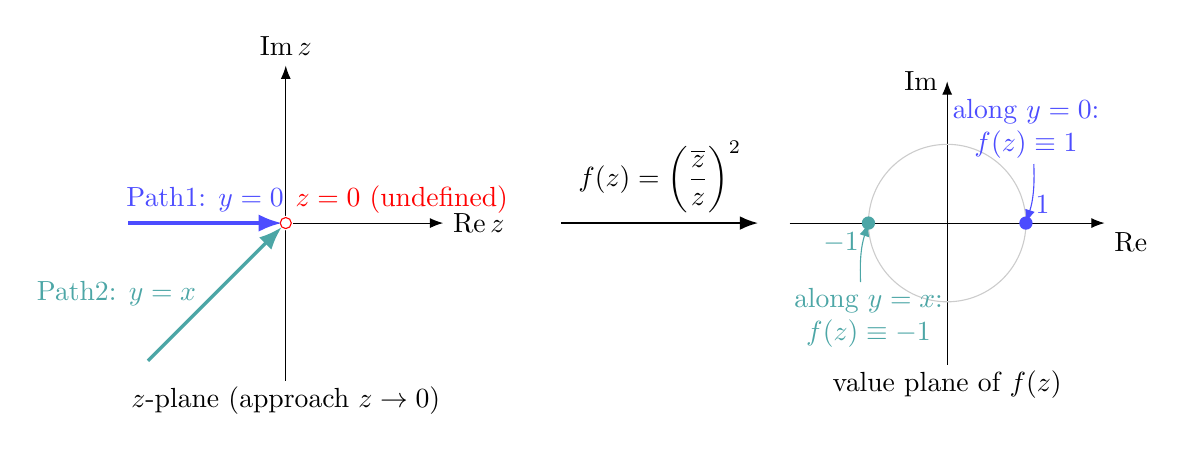
\begin{tikzpicture}[>=Latex,scale=1]
			% =============== z-plane (paths to the origin) ===============
			\begin{scope}
				% axes
				\draw[->] (-2.0,0) -- (2.0,0) node[right] {$\Re z$};
				\draw[->] (0,-2.0) -- (0,2.0) node[above] {$\Im z$};
				\node at (0,-2.25) {$z$-plane (approach $z\to 0$)};
				
				% origin as a hole (z=0 excluded)
				\fill[white] (0,0) circle (2.6pt);
				\draw[red] (0,0) circle (2pt) node[above right] {$z=0$ (undefined)};
				
				% Path 1: real axis y=0 (blue)
				\draw[blue!70,very thick,->] (-2,0) -- (-0.05,0) node[midway, above] {Path1: $y=0$};
				
				% Path 2: diagonal y=x (teal)
				\draw[teal!70,very thick,->] (-1.75,-1.75) -- (-0.05,-0.05) node[midway, xshift=-1.25cm] {Path2: $y=x$};
			\end{scope}
			% =============== mapping arrow ===============
			\draw[->,thick] (3.5,0) -- (6,0)
			node[midway,above] {$f(z)=\left(\dfrac{\overline z}{z}\right)^2$};
			% =============== value plane (outputs) ===============
			\begin{scope}[xshift=8.4cm]
				% axes
				\draw[->] (-2,0) -- (2,0) node[below right] {$\Re$};
				\draw[->] (0,-1.8) -- (0,1.8) node[left] {$\Im$};
				\node at (0,-2.05) {value plane of $f(z)$};
				
				% unit circle (context): |(\bar z/z)^2| = 1 for z≠0
				\draw[gray!40] (0,0) circle (1);
				
				% images of the two paths (constants 1 and -1)
				% Path 1 (y=0) -> 1
				\fill[blue!70] (1,0) circle (2.4pt) node[above right] {$1$};
				\draw[blue!70,->] (1.1,.75) to[bend left=10] (1,0);
				\node[blue!70,align=center] at (1,1.2)
				{along $y=0$:\\ $f(z)\equiv 1$};
				
				% Path 2 (y=x) -> -1
				\fill[teal!70] (-1,0) circle (2.4pt) node[below left] {$-1$};
				\draw[teal!70,->] (-1.1,-0.75) to[bend left=10] (-1,0);
				\node[teal!70,align=center] at (-1,-1.2)
				{along $y=x$:\\ $f(z)\equiv -1$};
				
				%	% conclusion box
				%	\node[draw,rounded corners=2pt,align=left,anchor=north] at (0,-1.25)
				%	{$\displaystyle \lim_{z\to 0}\left(\frac{\overline z}{z}\right)^2\ \text{does not exist},$\\
					%		since the limits along $y=0$ and $y=x$ differ.};
			\end{scope}
		\end{tikzpicture}
	\end{center}
	\medskip
	\noindent\textbf{(1) Path 1: approach along the real axis $y=0$}
	
	Let $z=x+0i=x$ with $x\in\mathbb{R}\setminus\{0\}$ and $x\to 0$. Then $
	\displaystyle\left(\frac{\overline{z}}{z}\right)^2
	=\left(\frac{x}{x}\right)^2
	=1$.
	
	\medskip
	\noindent\textbf{(2) Path 2: approach along the diagonal $y=x$}
	
	Let $z=x+ix=(1+i)x$ with $x\in\mathbb{R}\setminus\{0\}$ and $x\to 0$. Then
	\[
	\frac{\overline{z}}{z}
	=\frac{\overline{(1+i)x}}{(1+i)x}
	=\frac{(1-i)\,x}{(1+i)\,x}
	=\frac{1-i}{1+i}
	=\frac{(1-i)^2}{(1+i)(1-i)}
	=\frac{1-2i+i^2}{1- i^2}
	=\frac{1-2i-1}{2}
	=\frac{-2i}{2}
	=-i.
	\]
	Hence
	\[
	\left(\frac{\overline{z}}{z}\right)^2
	=(-i)^2
	=-1.
	\] 
	
	\medskip
	\noindent\textbf{(3) Conclusion}
	
	Since the limits along these two paths are different (namely $1$ and $-1$), the limit cannot exist.
\end{proof}

\begin{tcolorbox}
Let \[
f(z)=\begin{cases} \bar z^2/z,& z\neq0,\\ 0,& z=0.\end{cases}
\] Show that if $z=0$, then $\Delta w/\Delta z=1$ at eatch nonzero point on the real and imaginary axes in the $\Delta z$, or $\Delta x\Delta y$, plane. Then show that $\Delta w/\Delta z=-1$ at each nonzero point $(\Delta x, \Delta y)$ on the line $\Delta y=\Delta x$ in that plane. Conclude from these observations that $f'(0)$ does not exist. Note that to obtain this result, it is not sufficient to consider only horizontal and vertical approaches to the origin in the $\Delta z$ plane.
\end{tcolorbox}
\begin{proof}
	Let $\frac{\Delta w}{\Delta z}
	=\frac{f(\Delta z)-f(0)}{\Delta z}
	\quad(\Delta z\neq 0)$. Since $f(0)=0$, for $\Delta z\neq0$, $\displaystyle
	\frac{\Delta w}{\Delta z}
	=\frac{f(\Delta z)}{\Delta z}
	=\frac{\overline{\Delta z}^{\,2}}{(\Delta z)^2}$.
	
	\medskip
	\noindent\textbf{(1) Real and imaginary axes.}
	\begin{itemize}
		\item Real axis: $\Delta z=x$ with $x\in\mathbb{R}\setminus\{0\}$, $\displaystyle
		\frac{\Delta w}{\Delta z}=\frac{\overline{x}^{\,2}}{x^2}=\frac{x^2}{x^2}=1$.
		\begin{center}
			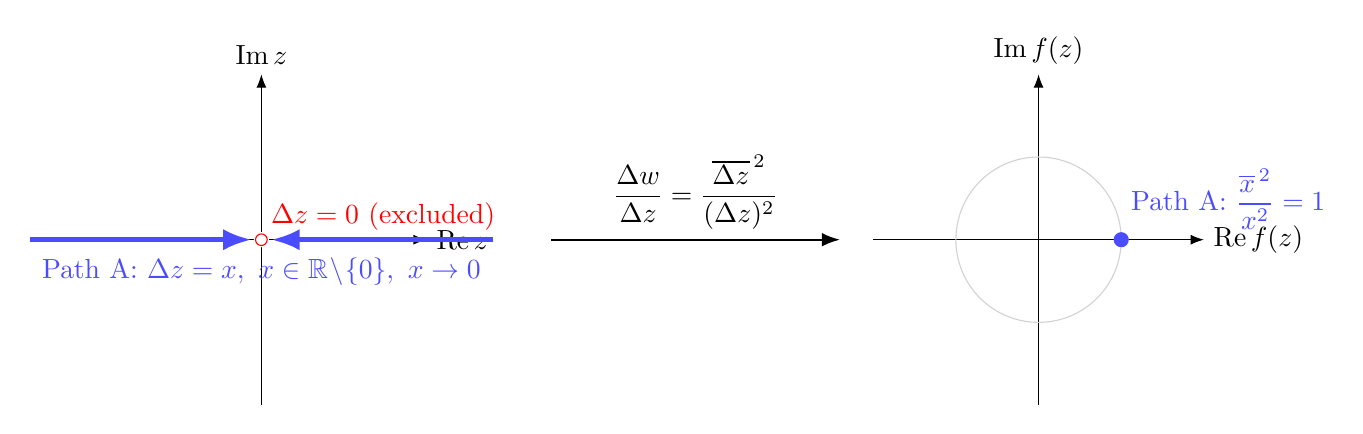
\begin{tikzpicture}[>=Latex,scale=1.05]	
				%================ z-plane: explicit paths =================
				\begin{scope}
					% axes
					\draw[->] (-2,0) -- (2,0) node[right] {$\Re z$};
					\draw[->] (0,-2) -- (0,2) node[above] {$\Im z$};
					% hole at the origin (Delta z = 0 excluded)
					\fill[white] (0,0) circle (2.6pt);
					\draw[red] (0,0) circle (2pt) node[above right] {$\Delta z=0$ (excluded)};
					% Path A: real axis, Δz = x, x→0, x≠0
					\draw[line width=1.6pt,blue!70,->] (-2.8,0) -- (-0.12,0);
					\draw[line width=1.6pt,blue!70,->] ( 2.8,0) -- ( 0.12,0);
					\node[blue!70,anchor=north] at (0,-0.10)
					{$\displaystyle \text{Path A: }\Delta z=x,\ x\in\mathbb R\!\setminus\!\{0\},\ x\to 0$};
				\end{scope}
				%================ mapping arrow =================
				\draw[->,thick] (3.5,0) -- (7,0)
				node[midway,above] {$\displaystyle \frac{\Delta w}{\Delta z}=\frac{\overline{\Delta z}^{\,2}}{(\Delta z)^2}$};
				%================ value plane: constant images =================
				\begin{scope}[xshift=9.4cm]
					% axes
					\draw[->] (-2,0) -- (2,0) node[right] {$\Re f(z)$};
					\draw[->] (0,-2) -- (0,2) node[above] {$\Im f(z)$};
					%	\node at (0,-2.55) {$f(z)$-plane of $\Delta w/\Delta z$};
					% unit circle for context (|Δw/Δz|=1 for Δz≠0)
					\draw[gray!35] (0,0) circle (1);
					% Image of Path A (real axis): constant 1
					\fill[blue!70] (1,0) circle (2.6pt) node[above right] {$\displaystyle \text{Path A: } \frac{\overline{x}^{\,2}}{x^2}=1$};
				\end{scope}
			\end{tikzpicture}
		\end{center}
		\item Imaginary axis: $\Delta z=iy$ with $y\in\mathbb{R}\setminus\{0\}$, $\displaystyle
		\frac{\Delta w}{\Delta z}
		=\frac{\overline{iy}^{\,2}}{(iy)^2}
		=\frac{(-iy)^2}{(iy)^2}
		=\frac{-y^2}{-y^2}=1$.
		\begin{center}
			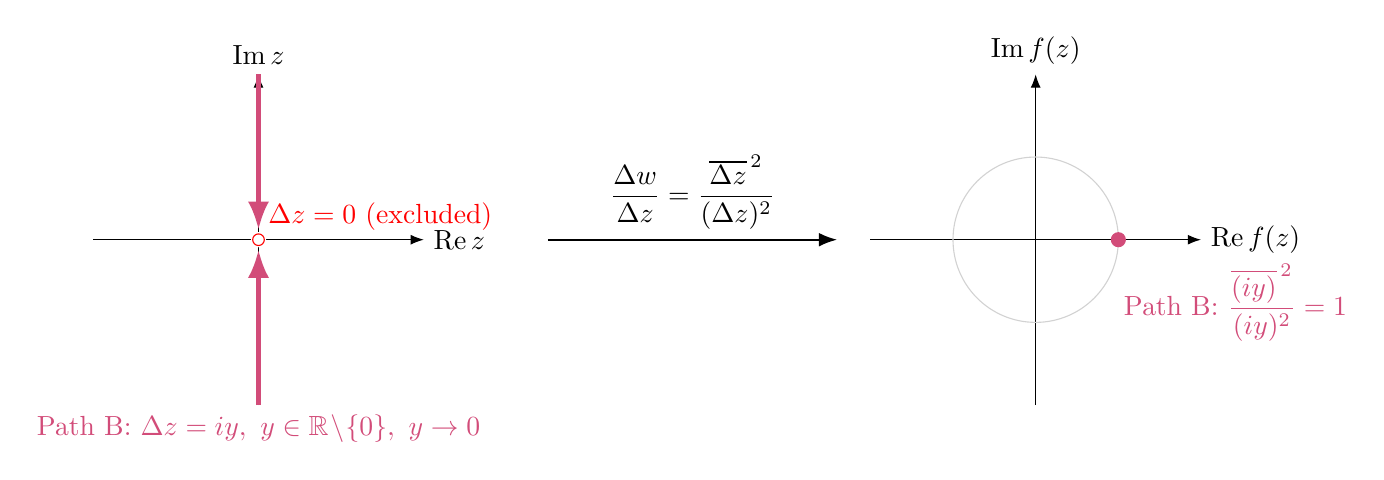
\begin{tikzpicture}[>=Latex,scale=1.05]	
				%================ z-plane: explicit paths =================
				\begin{scope}
					% axes
					\draw[->] (-2,0) -- (2,0) node[right] {$\Re z$};
					\draw[->] (0,-2) -- (0,2) node[above] {$\Im z$};
					% hole at the origin (Delta z = 0 excluded)
					\fill[white] (0,0) circle (2.6pt);
					\draw[red] (0,0) circle (2pt) node[above right] {$\Delta z=0$ (excluded)};
					% Path B: imaginary axis, Δz = iy, y→0, y≠0
					\draw[line width=1.6pt,purple!70,->] (0,-2.0) -- (0,-0.12);
					\draw[line width=1.6pt,purple!70,->] (0, 2.0) -- (0, 0.12);
					\node[purple!70,anchor=north] at (0,-2)
					{$\displaystyle \text{Path B: }\Delta z=iy,\ y\in\mathbb R\!\setminus\!\{0\},\ y\to 0$};
				\end{scope}
				%================ mapping arrow =================
				\draw[->,thick] (3.5,0) -- (7,0)
				node[midway,above] {$\displaystyle \frac{\Delta w}{\Delta z}=\frac{\overline{\Delta z}^{\,2}}{(\Delta z)^2}$};
				%================ value plane: constant images =================
				\begin{scope}[xshift=9.4cm]
					% axes
					\draw[->] (-2,0) -- (2,0) node[right] {$\Re f(z)$};
					\draw[->] (0,-2) -- (0,2) node[above] {$\Im f(z)$};
					%	\node at (0,-2.55) {$f(z)$-plane of $\Delta w/\Delta z$};
					% unit circle for context (|Δw/Δz|=1 for Δz≠0)
					\draw[gray!35] (0,0) circle (1);
					% Image of Path B (imag axis): constant 1
					\fill[purple!70] (1,0) circle (2.6pt);
					\node[purple!70,anchor=north west] at (0.95,-0.18)
					{$\displaystyle \text{Path B: } \frac{\overline{(iy)}^{\,2}}{(iy)^2}=1$};
				\end{scope}
			\end{tikzpicture}
		\end{center}
	\end{itemize}
	
	\noindent\textbf{(2) Line $\Delta y=\Delta x$.}
	Let $\Delta z=(1+i)x$ with $x\in\mathbb{R}\setminus\{0\}$. Then
	\[
	\frac{\Delta w}{\Delta z}
	=\frac{\overline{(1+i)x}^{\,2}}{((1+i)x)^2}
	=\frac{((1-i)x)^2}{((1+i)x)^2}
	=\frac{(1-i)^2}{(1+i)^2}
	=\frac{-2i}{2i}=-1.
	\]
	\begin{center}
		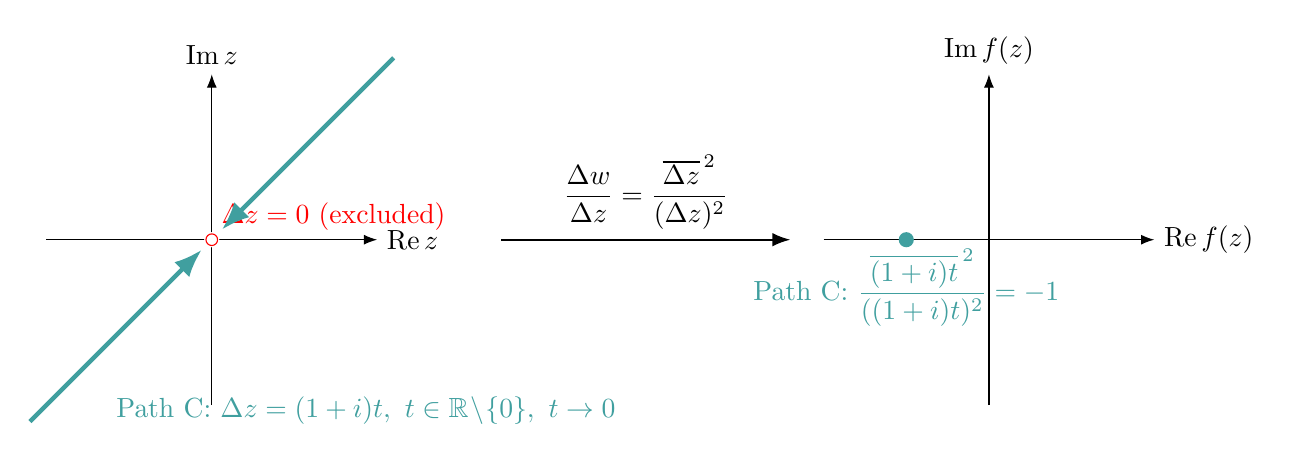
\begin{tikzpicture}[>=Latex,scale=1.05]	
			%================ z-plane: explicit paths =================
			\begin{scope}
				% axes
				\draw[->] (-2,0) -- (2,0) node[right] {$\Re z$};
				\draw[->] (0,-2) -- (0,2) node[above] {$\Im z$};
				%	\node at (0,-2.55) {$z$-plane (approach $\Delta z\to 0$)$\,$};	
				% hole at the origin (Delta z = 0 excluded)
				\fill[white] (0,0) circle (2.6pt);
				\draw[red] (0,0) circle (2pt) node[above right] {$\Delta z=0$ (excluded)};
				% Path C: diagonal Δy=Δx, i.e., Δz = (1+i)t, t→0, t≠0
				\draw[line width=1.6pt,teal!75,->] (-2.2,-2.2) -- (-0.12,-0.12);
				\draw[line width=1.6pt,teal!75,->] ( 2.2, 2.2) -- ( 0.12, 0.12);
				\node[teal!75,anchor=south east] at (5,-2.35)
				{$\displaystyle \text{Path C: }\Delta z=(1+i)t,\ t\in\mathbb R\!\setminus\!\{0\},\ t\to 0$};
			\end{scope}
			%================ mapping arrow =================
			\draw[->,thick] (3.5,0) -- (7,0)
			node[midway,above] {$\displaystyle 
				\frac{\Delta w}{\Delta z}=\frac{\overline{\Delta z}^{\,2}}{(\Delta z)^2}
				%	\displaystyle \,f(z)=\begin{cases}
					%		\overline z^{\,2}/z &\text{if}\; z\neq 0\\
					%		0 &\text{if}\; z=0
					%	\end{cases}
				$};
			%================ value plane: constant images =================
			\begin{scope}[xshift=9.4cm]
				% axes
				\draw[->] (-2,0) -- (2,0) node[right] {$\Re f(z)$};
				\draw[->] (0,-2) -- (0,2) node[above] {$\Im f(z)$};
				%	\node at (0,-2.55) {$f(z)$-plane of $\Delta w/\Delta z$};
				% Image of Path C (diagonal): constant -1
				\fill[teal!75] (-1,0) circle (2.6pt) node[below] {$\displaystyle \text{Path C: } \frac{\overline{(1+i)t}^{\,2}}{((1+i)t)^2}=-1$};
			\end{scope}
		\end{tikzpicture}
	\end{center}
	\medskip
	\noindent\textbf{(3) Conclusion.}
	Since the difference quotient equals $1$ along the axes but $-1$ along the line $\Delta y=\Delta x$, the limit
	\[
	\lim_{\Delta z\to 0}\frac{f(\Delta z)-f(0)}{\Delta z}
	\]
	depends on the path and therefore does not exist. Consequently, $f'(0)$ does not exist.
\end{proof}	
\vfill
\begin{tcolorbox}
Let \[
f(z)=\bar z,\quad f(z)=2x+ixy^2,\quad f(z)=e^{\bar z}
\] Then show that $f'(z)$ does not exists at any point.
\end{tcolorbox}
\begin{proof}[\Sol]
	Let \(z=x+iy\) and \(f(z)=u+iv\) with $x,y,u,v\in\R$. The Cauchy--Riemann equations \[
	u_x=v_y,\qquad u_y=-\,v_x
	\]
	are necessary and sufficient for complex differentiability.
	
	\medskip
	\noindent\textbf{(1) \(f_1(z)=\overline z=\overline{x+iy}=x-iy\).}
	
	Here \(u(x,y)=x,\ v(x,y)=-y\). Thus \[
	u_x=1,\quad u_y=0,\quad v_x=0,\quad v_y=-1.
	\]
	The CR require \(u_x=v_y\), i.e.\ \(1=-1\), which is impossible. Hence \(f_1'\) does not exist anywhere.
	
	\medskip\newpage
	\noindent\textbf{(2) \(f_2(z)=2x+i\,x y^{2}\).}
	
	Here \(u(x,y)=2x,\ v(x,y)=x y^{2}\). Thus
	\[
	u_x=2,\quad u_y=0,\quad v_x=y^{2},\quad v_y=2xy.
	\]
	The CR demand \[
	\begin{cases} u_x=v_y\\ u_y=-v_x \end{cases}\implies
	\begin{cases} 2=2xy\\ 0=y^2 \end{cases}\implies
	\begin{cases} xy=1\\ y=0 \end{cases}.
	\] These cannot hold simultaneously for any \(x\). Hence CR fail at every point, so \(f_2'\) exists nowhere.
	
	\medskip
	\noindent\textbf{(3) \(f_3(z)=e^{\overline z}\).}
	
	Let \(\overline z=x-iy\). Then $f_3(x,y)=e^{x-iy}=e^{x}(\cos y-i\sin y)$, so \[
	u(x,y)=e^{x}\cos y,\qquad v(x,y)=-\,e^{x}\sin y.
	\] Compute \[
	u_x=e^{x}\cos y,\quad u_y=-e^{x}\sin y,\quad
	v_x=-e^{x}\sin y,\quad v_y=-e^{x}\cos y.
	\] The CR give \[
	\begin{cases} u_x=v_y\\ u_y=-v_x \end{cases}\implies
	\begin{cases} e^x\cos y=-e^x\cos y\\ -e^x\sin y=+e^x\sin y \end{cases}\implies
	\begin{cases} \cos y = 0\\ \sin y=0 \end{cases}.
	\] These cannot hold simultaneously for any \(y\). Hence CR fail everywhere and \(f_3'\) exists nowhere.
\end{proof}

\vfill
\begin{tcolorbox}
Show that the function \[
f(z)=\ln r+i\theta\quad (r>0,\; 0<\theta<2\pi)
\] is analytic in the indicated domain of definition, with derivative $f'(z)=1/z$. Then show that th e composite function $g(z)=f(z^2+1)$ is analytic in the quadratic $x>0,y>0$ with derivative \[
g'(z)=\frac{2z}{z^2+1}.
\] (Suggestion: Observe that $\Im(z^2+1)>0$ when $x>0, y>0$)
\end{tcolorbox}
\begin{proof}[\sol]
	Let $z=x+iy=re^{i\theta}$ with $r=\sqrt{x^2+y^2}>0$ and $0<\theta<2\pi$. Define
	\[
	f(z)=\ln r+i\theta .
	\]
	Then $f$ is analytic on the slit plane
	\begin{center}
		\begin{minipage}{.475\textwidth} \[
			\Omega:=\{\,z\in\mathbb{C}: r>0,\ 0<\theta<2\pi\,\}=\mathbb{C}\setminus[0,\infty),
			\] and $f'(z)=\frac{1}{z}\; (z\in\Omega)$.
		\end{minipage}\hfill
		\begin{minipage}{.475\textwidth}\centering
			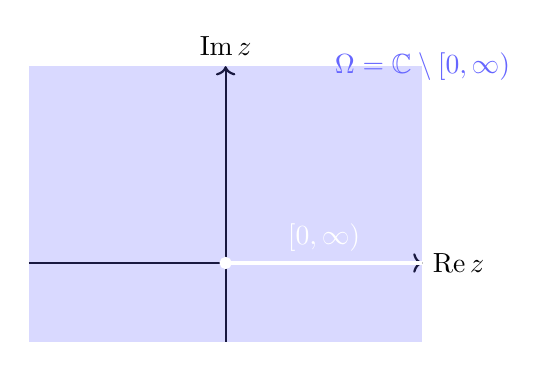
\begin{tikzpicture}
				% axes
				\draw[->, thick] (-2.5,0) -- (2.5,0) node[right] {$\Re z$};
				\draw[->, thick] (0,-1) -- (0,2.5) node[above] {$\Im z$};
				% shade domain
				\fill[blue!60, opacity=.25] (-2.5,-1) rectangle (2.5,2.5);
				\node[blue!60] at (2.5,2.5) {$\Omega=\C\setminus\intco{0,\infty}$};
				% slit: [0, +∞) on real axis
				\filldraw[white] (0,0) circle (2pt);
				\draw[white,ultra thick] (0,0) -- (2.5,0) node[midway, above] {$[0,\infty)$};
			\end{tikzpicture}
		\end{minipage}
	\end{center}
	Write $f=u+iv$ with \[
	u(x,y)=\ln r=\frac12\ln(x^2+y^2),\qquad v(x,y)=\theta=\Arg(z)\in(0,2\pi).
	\]
	On $\Omega$ the functions $u,v$ are $C^1$ and their partials are:
	\[
	u_x=\frac{x}{x^2+y^2},\quad u_y=\frac{y}{x^2+y^2},\qquad
	v_x=-\frac{y}{x^2+y^2},\quad v_y=\frac{x}{x^2+y^2}.
	\]
	Hence the Cauchy--Riemann equations hold on $\Omega$:
	\[
	u_x=v_y=\frac{x}{x^2+y^2},\qquad u_y=-v_x=\frac{y}{x^2+y^2}.
	\]
	Since these partials are continuous on $\Omega$, $f$ is analytic there. Its complex derivative is
	\[
	f'(z)=u_x+iv_x=\frac{x}{x^2+y^2}+i\!\left(-\frac{y}{x^2+y^2}\right)
	=\frac{x-iy}{x^2+y^2}=\frac{1}{x+iy}=\frac{1}{z}.
	\]
	For $g(z)=f(z^2+1)$, compute
	\begin{align*}
		z^2+1&=(x+iy)^2+1\\
		&=(x^2-y^2+2ixy) +1 \\
		&=(x^2-y^2+1)+i(2xy).
	\end{align*}
	If $x>0$ and $y>0$, then $\Im(z^2+1)=2xy>0$, so $z^2+1$ lies in the open upper half-plane $\mathbb{H}$, in particular in $\Omega$ (its argument lies in $(0,\pi)\subset(0,2\pi)$). Thus $g$ is the composition of analytic functions on the first quadrant $Q_1$, hence analytic on $Q_1$. By the chain rule, \[
	g'(z)=f'(z^2+1)\cdot(2z)=\frac{2z}{z^2+1}\qquad (z\in Q_1).
	\]
\end{proof}


\newpage
\section{Elementary functions}
\begin{tcolorbox}
Show that $f(z)=\exp(\overline{z})$ is not analytic anywhere. \textit{(Hint: use the Cauchy--Riemann equations.)}
\end{tcolorbox}
\begin{proof}[\sol]
	(\textbf{Proof via Cauchy--Riemann equations}) Write \(z=x+iy\). Then \[
	f(z)=e^{\overline z}=e^{x-iy}=e^{x}\bigl(\cos y-i\sin y\bigr),
	\] so \[
	u(x,y)=e^{x}\cos y,\qquad v(x,y)=-e^{x}\sin y.
	\] Then \[
	u_x=e^{x}\cos y,\quad u_y=-e^{x}\sin y,\qquad
	v_x=-e^{x}\sin y,\quad v_y=-e^{x}\cos y.
	\] If \(f\) is complex differentiable at \((x,y)\), the Cauchy--Riemann equations would hold: \[
	u_x=v_y \quad\text{and}\quad u_y=-\,v_x.
	\] That is, \begin{align*}
		u_x=v_y&\implies e^x\cos y=-e^x\cos y&\implies \cos y=0, \\
		u_y=-v_x&\implies -e^x\sin y=e^x\sin y&\implies \sin y=0.
	\end{align*}
	There is no \(y\in\mathbb{R}\) with \(\cos y=0\) and \(\sin y=0\) simultaneously. Hence the Cauchy--Riemann equations fail at every point, so \(f\) is nowhere analytic.
	
	\medskip\noindent
	(\textbf{Proof via Wirtinger derivatives})
	Using \(\partial/\partial z=\tfrac12(\partial_x- i\,\partial_y)\) and
	\(\partial/\partial\overline z=\tfrac12(\partial_x+ i\,\partial_y)\),
	one checks directly that \[
	\frac{\partial f}{\partial z}=0,
	\qquad
	\frac{\partial f}{\partial \overline z}=e^{\overline z}\neq 0\ \text{ for all } z.
	\]
	A function is holomorphic iff \(\partial f/\partial \overline z\equiv 0\) on its domain. Since this is not the case, \(f\) is nowhere holomorphic.
\end{proof}
\vfill
\begin{tcolorbox}
Show that $f(z)=\Log(z-i)$ is analytic except on portion $x\leq 0$ of the line $y=1$ and that the function
\[
f(z)=\frac{\Log(z+4)}{z^2+i}
\] is analytic everywhere except at the points $\pm{(1-i)}/{\sqrt2}$ and on the portion $x\leq -4$ of the real axis.
\end{tcolorbox}
\begin{proof}[\sol]
	Consider $\Log\; z=\ln|z|+i\Arg\; z$, the principal branch of the complex logarithm,
	with $\Arg\; z\in(-\pi,\pi)$, so that $\Log$ is analytic on \begin{align*}
		\mathbb{C}\setminus(-\infty,0] &= \C\setminus\set{z\in\C:\Re z\leq 0\land\Im z=0}\\
		&=\{\, z\in\mathbb{C} : \Re z>0\lor \Im z\neq 0\,\}.
	\end{align*} Then
	\begin{enumerate}[(1)]
		\item Since $\Log$ is analytic on $\mathbb{C}\setminus(-\infty,0]$ and the map $z\mapsto z-i$ is entire,
		the composition $z\mapsto \Log(z-i)$ is analytic precisely where $z-i\notin(-\infty,0]$.
		Equivalently, \begin{align*}
			z-i\in(-\infty,0] &\iff \Re(z-i)\le 0 \text{ and } \Im(z-i)=0 \\
			&\iff \Re(x+i(y-1))=x\le 0 \text{ and } \Im(x+i(y-1))=y-1=0.
		\end{align*}
		That is, $f(z):=\Log(z-i)$ is analytic on $\mathbb{C}\setminus\{\,x+iy:\; x\le 0,\ y=1\}$. 
		%i.e. it is analytic except on the portion $x\le0$ of the line $y=1$.
		\begin{center}
			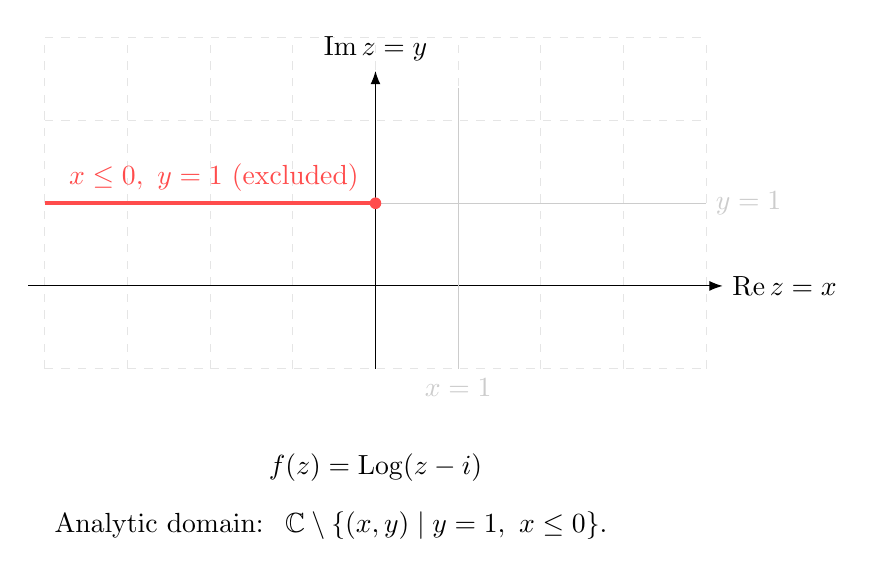
\begin{tikzpicture}[>=Latex,scale=1.05]
				\draw[gray!20, dashed] (-4,-1) grid (4,3);
				% axes
				\draw[->] (-4.2,0) -- (4.2,0) node[right] {$\Re z=x$};
				\draw[->] (0,-1) -- (0,2.6) node[above] {$\Im z=y$};
				\node at (0,-2.2) {$f(z)=\Log(z-i)$};
				% a few reference gridlines for context
				\draw[gray!40] (-4.0, 1.0) -- (4.0, 1.0) node[right] {$y=1$};
				\draw[gray!40] ( 1.0,2.4) -- ( 1.0, -1) node[below] {$x=1$};
				% branch cut in z-plane: y = 1, x <= 0  (comes from w=z-i \in (-\infty,0])
				\draw[ultra thick,red!70] (-4.0,1.0) -- (0.0,1.0) node[midway,above] {$\;x\le 0,\ y=1$ (excluded)};
				\fill[red!70] (0.0,1.0) circle (2pt); % includes endpoint x=0
				% legend
				\node[align=left,anchor=west] at (-4.0,-2.9)
				{Analytic domain: $\ \C \setminus \{(x,y)\mid y=1,\ x\le 0\}$.};
			\end{tikzpicture}
		\end{center}
		\item The numerator $z\mapsto \Log(z+4)$ is analytic wherever $z+4\notin(-\infty,0]$, i.e., $z\notin\intoc{-\infty,-4}$. In other words, $\Log(z+4)$ is analytic on \[
		\C\setminus\intoc{-\infty,-4}=\C\setminus\set{z\in\C:\Re z\leq -4\land \Im z = 0}=\set{z\in\C:\Re z>-4\lor \Im z\neq 0 }
		\] $\C\setminus\intoc{-\infty}$ for
		$z\notin(-\infty,-4]$, which is the portion $x\le -4$ of the real axis.
		The denominator $z^2+i$ vanishes exactly at the zeros of $z^2=-i$, namely
		\[
		z=\pm(-i)^{1/2}=\pm e^{-i\pi/4}=\pm\frac{1-i}{\sqrt2}.
		\]
		Therefore $g$ is analytic on the domain where the numerator is analytic and the denominator is nonzero, i.e.
		\[
		\mathbb{C}\setminus\Big( (-\infty,-4]\ \cup\ \{\pm\tfrac{1-i}{\sqrt2}\}\Big),
		\]
		which is exactly the stated set.
		
		$g(z):=\dfrac{\Log(z+4)}{z^2+i}$ is analytic on
		\[
		\mathbb{C}\setminus\Big(\{\,x+iy:\; y=0,\ x\le -4\,\}\ \cup\ \{\pm\tfrac{1-i}{\sqrt2}\}\Big),
		\]
		i.e. everywhere except at the branch cut $x\le -4$ on the real axis and at the two points $\pm{(1-i)}/{\sqrt2}$.
		
		\begin{center}
			\begin{tikzpicture}[>=Latex,scale=1.05]
%				\draw[gray!20, dashed] (-4,-4) grid (4,4);
				% axes
				\draw[->] (-6.2,0) -- (4.2,0) node[right] {$\Re z=x$};
				\draw[->] (0,-1.2) -- (0,3.2) node[above] {$\Im z=y$};
%				\node at (0,-3.5) {$g(z)=\dfrac{\Log(z+4)}{z^2+i}$};
				% branch cut from Log(z+4): real axis x <= -4
				\draw[very thick,red!70] (-6.0,0.0) -- (-4.0,0.0) node[midway,above] {$\ (-\infty,-4]$ (excluded)};
				\fill[red!70] (-4.0,0.0) circle (2pt); % includes endpoint x=-4
				% poles from z^2+i=0: z = ±(1 - i)/√2  ≈ (±0.7071, ∓0.7071)
				\draw[red!80,very thick] ( 0.7071,-0.7071) +(0.12,0.12) -- +(-0.12,-0.12);
				\draw[red!80,very thick] ( 0.7071,-0.7071) +(-0.12,0.12) -- +(0.12,-0.12);
				\node[red!80,anchor=west] at (0.78,-0.70) {$\ \ \tfrac{1-i}{\sqrt2}$};
				\draw[red!80,very thick] (-0.7071, 0.7071) +(0.12,0.12) -- +(-0.12,-0.12);
				\draw[red!80,very thick] (-0.7071, 0.7071) +(-0.12,0.12) -- +(0.12,-0.12);
				\node[red!80,anchor=east] at (-0.78,0.70) {$\tfrac{-1+i}{\sqrt2}\ $};
				\draw[red!80,very thick, dotted] ( 0.7071,0) -- ( 0.7071,-0.7071);
				\draw[red!80,very thick, dotted] ( 0,-0.7071) -- ( 0.7071,-0.7071);
				\draw[red!80,very thick, dotted] ( -0.7071,0.7071) -- ( -0.7071,0);
				\draw[red!80,very thick, dotted] ( 0,0.7071) -- ( -0.7071,0.7071);
				%					% legend
				%					\node[align=left,anchor=west] at (-6.0,-2.7)
				%					{Analytic domain: $\ \C\setminus\big((-\infty,-4]\cup\{\pm\tfrac{1-i}{\sqrt2}\}\big)$.};
			\end{tikzpicture}
		\end{center}
	\end{enumerate}
\end{proof}

\begin{tcolorbox}
Show that the function $\ln(x^2+y^2)$ is harmonic in every domain that does not contain the origin.
\end{tcolorbox}
\begin{proof}[\sol]
	%		We need to show that $u(x,y) = \ln(x^2 + y^2)$
	%		satisfies Laplace’s equation \[
	%		u_{xx} + u_{yy} = 0
	%		\] at every point $(x,y)\neq(0,0)$. 
	For $(x,y)\neq(0,0)$, we can differentiate: \begin{align*}
		u_x &= \frac{\partial}{\partial x}\ln(x^2 + y^2) = \frac{2x}{x^2 + y^2},\\
		u_y &= \frac{\partial}{\partial y}\ln(x^2 + y^2) = \frac{2y}{x^2 + y^2}.
	\end{align*} And then \begin{align*}
		u_{xx}
		&= \frac{2(x^2 + y^2) - 2x\cdot 2x}{(x^2 + y^2)^2}
		= \frac{2(x^2 + y^2) - 4x^2}{(x^2 + y^2)^2}
		= \frac{-2x^2 + 2y^2}{(x^2 + y^2)^2} \\
		u_{yy}
		&= \frac{2(x^2 + y^2) - 2y\cdot 2y}{(x^2 + y^2)^2}
		= \frac{2(x^2 + y^2) - 4y^2}{(x^2 + y^2)^2}
		= \frac{2x^2 - 2y^2}{(x^2 + y^2)^2}.
	\end{align*}	
	Now compute the Laplacian: \[
	u_{xx} + u_{yy}
	= \frac{-2x^2 + 2y^2}{(x^2 + y^2)^2}+
	\frac{2x^2 - 2y^2}{(x^2 + y^2)^2}
	= \frac{(-2x^2 + 2y^2) + (2x^2 - 2y^2)}{(x^2 + y^2)^2}
	= \frac{0}{(x^2 + y^2)^2}
	= 0
	\] for all $(x,y)\neq(0,0)$.
	%		So $\ln(x^2 + y^2)$ is harmonic at every point where it is twice continuously differentiable --- that is, on any domain that does not contain the origin (since at ((0,0)) the function is not even defined, and our derivatives blow up).	
	%		Therefore, **(\ln(x^2 + y^2)) is harmonic in every domain that does not contain the origin.**
	
	\medskip\noindent
	(\textbf{Proof via Wirtinger-operator})
	Let $z=x+iy$ and
	\[
	u(x,y)=\ln(x^2+y^2)=\ln(\abs{z}^2)=\ln(z\bar z).
	\]
	Recall the Wirtinger operators $
	\partial:=\tfrac12(\partial_x-i\,\partial_y)$ and
	$\bar\partial:=\tfrac12(\partial_x+i\,\partial_y),$
	so that the Laplacian satisfies
	\[
	\Delta=\partial_{xx}+\partial_{yy}=4\,\partial\bar\partial=4\,\bar\partial\partial.
	\]
	On $\mathbb{C}\setminus\{0\}$ the chain rule gives \begin{align*}
		\partial u
		&=\partial\big(\ln(z\bar z)\big)
		=\frac{1}{z\bar z}\,\partial(z\bar z)
		=\frac{1}{z\bar z}\,\bar z
		=\frac{1}{z},\\
		\bar\partial u
		&=\bar\partial\big(\ln(z\bar z)\big)
		=\frac{1}{z\bar z}\,\bar\partial(z\bar z)
		=\frac{1}{z\bar z}\,z
		=\frac{1}{\bar z}.
	\end{align*}
	Therefore, $\displaystyle
	\Delta u
	=4\,\partial\bar\partial u
	=4\,\partial\!\left(\frac{1}{\bar z}\right)
	=0$ on $\mathbb{C}\setminus\{0\}$. 
\end{proof}

\begin{tcolorbox}
Show that $\cosh^2 z-\sinh^2 z=1$ and $\sinh z+\cosh z=e^z$.
\end{tcolorbox}
\begin{proof}[\sol]
	Recall the exponential definitions (valid for all $z\in\mathbb{C}$):
	\[
	\cosh z=\frac{e^{z}+e^{-z}}{2},\qquad
	\sinh z=\frac{e^{z}-e^{-z}}{2}.
	\]
	
	\medskip
	\noindent\textbf{(1) $\cosh^2 z-\sinh^2 z=1$.}
	\[
	\cosh^2 z-\sinh^2 z
	=\left(\frac{e^{z}+e^{-z}}{2}\right)^{\!2}
	-\left(\frac{e^{z}-e^{-z}}{2}\right)^{\!2}
	=\frac{(e^{z}+e^{-z})^2-(e^{z}-e^{-z})^2}{4}.
	\]
	Expanding,
	\[
	(e^{z}+e^{-z})^2-(e^{z}-e^{-z})^2
	=e^{2z}+2+e^{-2z}-(e^{2z}-2+e^{-2z})=4,
	\]
	so $\cosh^2 z-\sinh^2 z=\frac{4}{4}=1$.
	
	\medskip
	\noindent\textbf{(2) $\sinh z+\cosh z=e^{z}$.}
	\[
	\sinh z+\cosh z
	=\frac{e^{z}-e^{-z}}{2}+\frac{e^{z}+e^{-z}}{2}
	=e^{z}.
	\]
\end{proof}


\newpage
\section{Integrals}
\begin{tcolorbox}
Let $C_0$ be the positively oriented circle $|z-z_0|=R$. Show that \[
\int_{C_0} (z - z_0)^{n-1}\,\d z =
\begin{cases}
		0, & n=\pm1,\pm2,\dots \\
		2\pi i, & n=0.
	\end{cases}
\]
\end{tcolorbox}
\begin{proof}[\sol]
Parametrize $C_0$ by $
z(t)=z_0+Re^{it}$ ($t\in[0,2\pi]$) then $dz=iRe^{it}\,\d t$ and
\[
\int_{C_0} (z-z_0)^{\,n-1}\,\d z
=\int_{0}^{2\pi} (Re^{it})^{\,n-1}\, iRe^{it}\,\d t
= iR^{n}\int_{0}^{2\pi} e^{int}\,\d t.
\] \begin{enumerate}[(1)]
		\item If $n\neq0$, then \[
		\int_{0}^{2\pi} e^{int}\,\d t=\left[\frac{1}{in}e^{int}\right]_{0}^{2\pi}=\frac{e^{in2\pi}-1}{in}=\frac{1-1}{in}=0,\qquad\text{so the integral is $0$.}
		\] 
		\item If $n=0$, then $e^{int}\equiv 1$ and the integral equals $iR^{0}\int_{0}^{2\pi} 1\,\d t=2\pi i$.
	\end{enumerate}
\end{proof}

\begin{tcolorbox}
Let $C$ be the boundary of the square with sides $x=\pm 2$, $y=\pm 2$, oriented positively. Show that
\[
\int_C \frac{\cos z}{z(z^2+8)}\,dz = \frac{i\pi}{4},\qquad
\int_C \frac{\cosh z}{z^4}\,dz = 0,\qquad
\int_C \frac{\tan(z/2)}{(z-x_0)^2}\,dz = i\pi \sec^2\!\left(\frac{x_0}{2}\right),
\] where $-2<x_0<2$.
\end{tcolorbox}
\begin{proof}[\sol]
Let $C$ be the positively oriented boundary of the square $\{x+iy:\ |x|\le2,\ |y|\le2\}$.
\begin{center}
\begin{tikzpicture}[scale=.9]
\tikzset{
		axis/.style={black, line cap=round, -Stealth},
		box/.style={thick, blue!65},
		orient/.style={-{Latex}, blue!65, thick}
	}
\draw[axis] (-3.0,0) -- (3.0,0) node[right] {$\Re z$};
\draw[axis] (0,-3.0) -- (0,3.0) node[above] {$\Im z$};
% square boundary |x|<=2, |y|<=2
\draw[box] (-2,-2) rectangle (2,2);
% CCW orientation arrows (midpoints of edges)
\draw[orient] ( 0, 2) -- ++(-1.1,0);
\draw[orient] ( 2, 0) -- ++(0,1.1);
\draw[orient] ( 0,-2) -- ++(1.1,0);
\draw[orient] (-2, 0) -- ++(0, -1.1);
\end{tikzpicture}
\end{center}
\begin{enumerate}[(1)]
\item $\displaystyle \int_C \frac{\cos z}{z(z^2+8)}\,dz$.\quad
The integrand is meromorphic with simple poles at $z=0$ and $z=\pm 2\sqrt2\,i$. Only $z=0$ is inside $C$. Around $z=0$, \[
\cos z=1-\frac{z^2}{2}+\frac{z^4}{4!}-\cdots,\qquad
\frac{1}{z(z^2+8)}=\frac{1}{z^3+8z}=\frac{1}{8z}\,\frac{1}{1+z^2/8}
=\frac{1}{8z}\Bigl(1-\frac{z^2}{8}+\frac{z^4}{8^2}-\cdots\Bigr).
\] Thus, \[
\Res_{z=0}\frac{\cos z}{z(z^2+8)}
=\Res_{z=0}\left(\frac{1}{8z}\Bigl(1-\frac{z^2}{8}+\frac{z^4}{8^2}-\cdots\Bigr)\Bigl(1-\frac{z^2}{2}+\frac{z^4}{4!}-\cdots\Bigr)\right)
%		=\lim_{z\to0}\frac{\cos z}{z^2+8}
=\frac{1}{8}.
\]
By the residue theorem,
\[
\int_C \frac{\cos z}{z(z^2+8)}\,dz
=2\pi i\cdot\frac18
=\frac{i\pi}{4}.
\]
\item $\displaystyle \int_C \frac{\cosh z}{z^4}\,dz$.\quad
Here the only singularity is at $z=0$ (order $4$).
Using
\[
\cosh z=1+\frac{z^2}{2!}+\frac{z^4}{4!}+\cdots,
\qquad
\frac{\cosh z}{z^4}=\frac{1}{z^4}+\frac{1}{2}\frac{1}{z^2}+\frac{1}{4!}+\cdots,
\]
there is no $1/z$ term; hence $\Res_{z=0}(\cosh z/z^4)=0$, and therefore
\[
\int_C \frac{\cosh z}{z^4}\,dz=0.
\]
\item $\displaystyle \int_C \frac{\tan(z/2)}{(z-x_0)^2}\,dz$ with $-2<x_0<2$.\quad 	We know that \[
\tan w = \frac{\sin w}{\cos w},
\] so the poles of $\tan w$ occur exactly where $\cos w = 0$ and $\sin w \neq 0$. The zeros of $\cos w$ are \[
w = \frac{\pi}{2} + k\pi = \frac{(2k+1)\pi}{2}, \quad k \in \mathbb{Z}.
\] Now consider $\tan\!\left(\frac{z}{2}\right)$. Let $
w = \frac{z}{2}$. The poles of $\tan(z/2)$ occur where $w$ is a pole of $\tan w$, i.e.\ where
\[
\frac{z}{2} = \frac{(2k+1)\pi}{2}, \quad k \in \mathbb{Z}.
\] So the poles of $\tan(z/2)$ are precisely at $z = (2k+1)\pi$ with $k\in\mathbb{Z}$. Since \[
|(2k+1)\pi| \ge \pi > 2,
\]
none of these poles lie inside or on $C$. Hence $\tan(z/2)$ is analytic on and inside $C$. The only singularity of the integrand ${\tan(z/2)}/{(z - x_0)^2}$ inside $C$ is at $z = x_0$.
Since $\tan(z/2)$ is analytic at $z = x_0$, we may expand it in a Taylor series about $x_0$: \begin{align*}
	\tan\!\left(\frac{z}{2}\right)
	&= \tan\!\left(\frac{x_0}{2}\right)
	+ \left.\frac{\d}{\d z}\tan\left(\frac{z}{2}\right)\right|_{z = x_0} (z - x_0)
	+ \cdots\\
	&=\tan\!\left(\frac{x_0}{2}\right)
	+ \frac12 \sec^2\!\left(\frac{x_0}{2}\right) (z - x_0)
	+ \cdots.
\end{align*}
Dividing by $(z - x_0)^2$ gives the Laurent series
\[
\frac{\tan(z/2)}{(z - x_0)^2}
= \frac{\tan(x_0/2)}{(z - x_0)^2}
+ \frac12 \sec^2\!\left(\frac{x_0}{2}\right)\frac{1}{z - x_0}
+ \cdots.
\] Thus, we obtain \[
\operatorname{Res}_{z=x_0}\!\left(\frac{\tan(z/2)}{(z - x_0)^2}\right)
= \frac12 \sec^2\!\left(\frac{x_0}{2}\right).
\]
By the residue theorem,
\[
\int_C \frac{\tan(z/2)}{(z - x_0)^2}\,dz
= 2\pi i \cdot \frac12 \sec^2\!\left(\frac{x_0}{2}\right)
= i\pi \sec^2\!\left(\frac{x_0}{2}\right).
\]
\end{enumerate}
\end{proof}

\newpage
\section{Series}
\begin{tcolorbox}
Show that the limit of a convergent complex sequence is unique by appealing to the corresponding result for a sequence of real numbers.
\end{tcolorbox}
\begin{proof}[\sol]
	We want to show that \begin{center}
		``If a complex sequence $\set{z_n}$ converges to both $L$ and $M$ in $\mathbb{C}$, then $L=M$.''
	\end{center}
	Write $z_n=x_n+iy_n$, $L=a+ib$, $M=c+id$ with $x_n,y_n,a,b,c,d\in\mathbb{R}$.
	Assume that \[
	z_n\to L\quad\text{and}\quad z_n\to M
	\] as $n\to\infty$. Taking real and imaginary parts, \[
	x_n=\Re z_n \to \Re L=a \quad\text{and}\quad x_n=\Re z_n \to \Re M=c,
	\] \[
	y_n=\Im z_n \to \Im L=b \quad\text{and}\quad y_n=\Im z_n \to \Im M=d.
	\]
	By the \emph{uniqueness of limits for real sequences}, these imply $a=c$ and $b=d$. Hence \[
	L=a+ib=c+id=M.
	\]
\end{proof}

\begin{tcolorbox}
Show that \[
\sum_{n=1}^{\infty} z_n=S\implies \sum_{n=1}^{\infty} \overline{z_n}=\overline{S}.
\]
\end{tcolorbox}
\begin{proof}[\sol]
	Let $s_N:=\sum_{n=1}^{N} z_n$ be the partial sums. By hypothesis $s_N\to S$ as $N\to\infty$.
	Consider the conjugated partial sums
	\[
	\overline{s_N}=\overline{\sum_{n=1}^{N} z_n}=\sum_{n=1}^{N}\overline{z_n},
	\]
	so $\{\overline{s_N}\}$ are the partial sums of $\sum_{n=1}^{\infty}\overline{z_n}$.
	Since complex conjugation is continuous (indeed, an isometry: $|\overline{w}-\overline{z}|=|w-z|$),
	we have $\overline{s_N}\to\overline{S}$. Therefore the series $\sum_{n=1}^{\infty}\overline{z_n}$ converges and
	\[
	\sum_{n=1}^{\infty}\overline{z_n}=\lim_{N\to\infty}\sum_{n=1}^{N}\overline{z_n}
	=\lim_{N\to\infty}\overline{s_N}=\overline{S}.
	\]
\end{proof}

\newpage
\begin{tcolorbox}
Derive the Taylor series representation \[
\frac{1}{1-z}=\sum_{n=0}^{\infty}\frac{(z-i)^n}{(1-i)^{\,n+1}},\qquad |z-i|<\sqrt{2}.
\] 
\end{tcolorbox}
\begin{proof}[\sol]
	Note that \[
	\frac{1}{1-z}
	=\frac{1}{(1-i)-(z-i)}
	=\frac{1}{1-i}\cdot\frac{1}{1-\left(\frac{z-i}{1-i}\right)}.
	\] For \(\left|\dfrac{z-i}{1-i}\right|<1\) (i.e. \(|z-i|<|1-i|=\sqrt{2}\)), expand the geometric series:
	\[
	\frac{1}{1-w}=\sum_{n=0}^{\infty} w^{n}\quad (|w|<1),\qquad
	w=\frac{z-i}{1-i}.
	\] Hence \[
	\frac{1}{1-z}
	=\frac{1}{1-i}\sum_{n=0}^{\infty}\left(\frac{z-i}{1-i}\right)^n
	=\sum_{n=0}^{\infty}\frac{(z-i)^n}{(1-i)^{\,n+1}},
	\]
	which converges for \(|z-i|<\sqrt{2}\).
	
	\medskip
	
	\begin{center}
		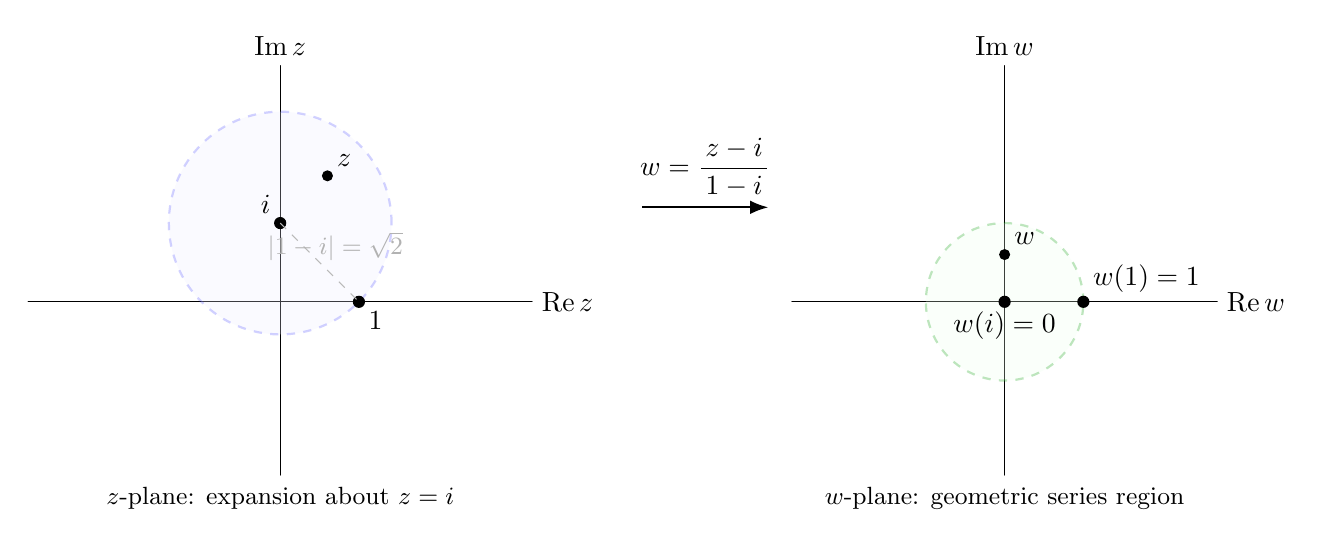
\begin{tikzpicture}[>=Latex,scale=1]
			\tikzset{
				axis/.style={black, line cap=round},
				disk/.style={draw=blue!70, fill=blue!8, thick, opacity=.25, dashed},
				unit/.style={draw=green!60!black, fill=green!8, thick, opacity=.25, dashed},
				note/.style={gray!60, font=\small},
				title/.style={font=\small},
				point/.style={black, fill=black},
				maparrow/.style={-{Latex}, thick}
			}
			% ================= LEFT: z-plane =================
			\begin{scope}
				% axes
				\draw[axis] (-3.2,0) -- (3.2,0) node[right] {$\Re z$};
				\draw[axis] (0,-2.2) -- (0,3.0) node[above] {$\Im z$};
				\node[title] at (0,-2.5) {$z$-plane: expansion about $z=i$};
				% disk centered at i with radius sqrt(2)
				\def\R{1.4142}
				\draw[disk] (0,1) circle (\R);
				% key points: i and 1
				\fill[point] (0,1) circle (2.2pt) node[above left] {$i$};
				\fill[point] (1,0) circle (2.2pt) node[below right] {$1$};	
				% show that 1 is on the boundary: |1-i|=sqrt(2)
				\draw[gray!55,dashed] (0,1) -- (1,0);
				\node[note] at (0.7,0.7) {$|1-i|=\sqrt{2}$};	
				% a sample z inside the disk
				\coordinate (Z) at (0.6,1.6);
				\fill (Z) circle (2.0pt) node[above right] {$z$};
			\end{scope}
			% mapping arrow
			\draw[maparrow] (4.6,1.2) -- (6.2,1.2)
			node[midway,above] {$\displaystyle w=\frac{z-i}{\,1-i\,}$};
			
			% ================= RIGHT: w-plane =================
			\begin{scope}[xshift=9.2cm]
				% axes
				\draw[axis] (-2.7,0) -- (2.7,0) node[right] {$\Re w$};
				\draw[axis] (0,-2.2) -- (0,3) node[above] {$\Im w$};
				\node[title] at (0,-2.5) {$w$-plane: geometric series region};
				
				% unit disk |w|<1
				\draw[unit] (0,0) circle (1);
				
				% images of key points: i -> 0, 1 -> 1
				\fill[point] (0,0) circle (2.2pt) node[below] {$w( i)=0$};
				\fill[point] (1,0) circle (2.2pt) node[above right] {$w(1)=1$};
				
				% image of sample z
				% For Z=(0.6,1.6): z-i=(0.6,0.6), 1-i=(1,-1) so w=(0.6+0.6i)/(1-i)=0.6i
				\coordinate (W) at (0,0.6);
				\fill (W) circle (2.0pt) node[above right] {$w$};
			\end{scope}
		\end{tikzpicture}
	\end{center}
\end{proof}

\begin{tcolorbox}
Show that the two Laurent series in powers of $z$ that represent the function \[
f(z)=\frac{1}{z(1+z^2)}
\] are\[
\sum_{n=0}^{\infty}(-1)^{n+1} z^{2n+1}+\frac{1}{z}\quad(0<|z|<1),
\qquad
\sum_{n=1}^{\infty}\frac{(-1)^{n+1}}{z^{2n+1}}\quad(1<|z|<\infty).
\]
\end{tcolorbox}
\begin{proof}[\sol]
	\begin{enumerate}[(1)]
		\item (\(0<|z|<1\))\quad Since \[
		\frac{1}{1+z^2}=\frac{1}{1-(-z^2)}=\sum_{n=0}^\infty (-z^2)^n=\sum_{n=0}^\infty (-1)^n z^{2n}\qquad(|z|<1),
		\] we have \begin{align*}
			\frac{1}{z(1+z^2)}=\frac{1}{z}\sum_{n=0}^\infty (-1)^n z^{2n}
			&=\sum_{n=0}^\infty (-1)^n z^{2n-1}\\
			&=\frac{1}{z}+\left(-z\right)+z^3+(-z^5)+z^7+\cdots\\
			&=\frac{1}{z}+\sum_{n=0}^\infty (-1)^{n+1} z^{2n+1}.
		\end{align*}
		Therefore the Laurent series on \(0<|z|<1\) is $\displaystyle \sum_{n=0}^{\infty}(-1)^{n+1} z^{2n+1}+\frac{1}{z}$.
		\item (\(1<|z|<\infty\))\quad Since \[
		\frac{1}{1+z^2}=\frac{1}{z^2}\,\frac{1}{1+z^{-2}}=\frac{1}{z^2}\,\frac{1}{1-(-z^{-2})}
		=\frac{1}{z^2}\sum_{n=0}^\infty (-1)^n z^{-2n}\qquad(|z|>1),
		\] we obtain \begin{align*}		
			\frac{1}{z(1+z^2)}=\frac{1}{z}\cdot\frac{1}{z^2}\sum_{n=0}^\infty (-1)^n z^{-2n}
			&=\sum_{n=0}^\infty \frac{(-1)^n}{z^{2n+3}}\\
			&=\frac{1}{z^3}+\frac{-1}{z^5}+\frac{1}{z^7}+\frac{-1}{z^9}+\cdots \\
			&=\sum_{n=1}^\infty \frac{(-1)^{n+1}}{z^{2n+1}},
		\end{align*} Hence the Laurent series is $\displaystyle \sum_{n=1}^{\infty}\frac{(-1)^{n+1}}{z^{2n+1}}$ on \(1<|z|<\infty\).
	\end{enumerate} 
\end{proof}

\begin{tcolorbox}
 Let $a\in\R$, where $-1<a<1$. Then the Laurent series representation $a/(z-a)$ is \[
\frac{a}{z-a}=\sum_{n=1}^{\infty}\frac{a^{n}}{z^{n}},\qquad |a|<|z|<\infty.
\]
After writing $z=e^{i\theta}$ in the above equation, equate real parts and then imaginary parts on each side of the result to derive the summation formulas:
\[
\sum_{n=1}^{\infty} a^n \cos(n\theta)=\frac{a\cos\theta-a^2}{1-2a\cos\theta+a^2}\quad\text{and}\quad
\sum_{n=1}^{\infty} a^n \sin(n\theta)=\frac{a\sin\theta}{1-2a\cos\theta+a^2}.
\]
\end{tcolorbox}
	\begin{proof}[\sol]
	For $|a|<|z|$, we know that
	\[
	\frac{a}{z-a}
	=\frac{a}{z}\,\frac{1}{1-a/z}
	=\frac{a}{z}\,\sum_{n=0}^\infty\left(\frac{a}{z}\right)^n
	=\sum_{n=0}^\infty\left(\frac{a}{z}\right)^{n+1}
	=\sum_{n=1}^{\infty}\frac{a^{n}}{z^{n}}.
	\] Set $z=e^{i\theta}$ (so $|a|<|z|=1$). Then
	\[
	\frac{a}{e^{i\theta}-a}=\sum_{n=1}^{\infty} a^n e^{-in\theta}
	=\sum_{n=1}^{\infty} a^n\bigl(\cos(n\theta)-i\sin(n\theta)\bigr).
	\]
	Note that \begin{align*}
		\frac{a}{e^{i\theta}-a}
		=\frac{e^{-i\theta}}{e^{-i\theta}}\cdot\frac{a}{e^{i\theta}-a}
		=\frac{a e^{-i\theta}}{1-a e^{-i\theta}}
		=\frac{a e^{-i\theta}(1-a e^{i\theta})}{(1-a e^{i\theta})(1-a e^{-i\theta})}
		&=\frac{a e^{-i\theta}(1-a e^{i\theta})}{1-a(e^{i\theta}+e^{-i\theta})+a^2e^{i\theta-i\theta}}\\
		&=\frac{a\,(e^{-i\theta}-a)}{1-2a\cos\theta+a^2}\\
		&=\frac{a\,(\cos\theta-i\sin\theta-a)}{1-2a\cos\theta+a^2}\\
		&=\frac{a(\cos\theta-a)-i\,a\sin\theta}{1-2a\cos\theta+a^2}.
	\end{align*} Thus, we obtain \[
	\sum_{n=1}^{\infty} a^n\bigl(\cos(n\theta)-i\sin(n\theta)\bigr)=\frac{a}{e^{i\theta}-a}=\frac{a(\cos\theta-a)-i\,a\sin\theta}{1-2a\cos\theta+a^2}.
	\] Therefore \[
	\sum_{n=1}^{\infty} a^n \cos(n\theta)=\frac{a\cos\theta-a^2}{1-2a\cos\theta+a^2},\qquad
		\sum_{n=1}^{\infty} a^n \sin(n\theta)=\frac{a\sin\theta}{1-2a\cos\theta+a^2},
	\]
	valid for $-1<a<1$ (indeed $1-2a\cos\theta+a^2=(1-a e^{i\theta})(\overline{1-a e^{i\theta}})=|1-ae^{i\theta}|^2>0$).
\end{proof}

\begin{tcolorbox}
With the aid of series, show that the function $f$ defined by means of the equations \[
f(z)=\begin{cases}
	(\sin z)/z &: z\neq 0\\
	1 &: z = 0
\end{cases}\] is entire. Use this result to establish the limit \[
\lim_{z\to0}\frac{\sin z}{z}=1.
\]
\end{tcolorbox}
\begin{proof}[\sol]
	The Maclaurin series of $\sin z$ (entire) is
	\[
	\sin z=\sum_{n=0}^{\infty}(-1)^n\frac{z^{2n+1}}{(2n+1)!}\,.
	\]
	For $z\neq 0$, divide by $z$:
	\[
	\frac{\sin z}{z}=\sum_{n=0}^{\infty}(-1)^n\frac{z^{2n}}{(2n+1)!}
	=1-\frac{z^{2}}{3!}+\frac{z^{4}}{5!}-\cdots .
	\]
	This is a power series with infinite radius of convergence, hence defines an entire function
	\[
	F(z):=\sum_{n=0}^{\infty}(-1)^n\frac{z^{2n}}{(2n+1)!}.
	\]
	Note that $F(0)=1$, and for $z\neq 0$ we have $F(z)=\sin z/z$. Therefore $f\equiv F$ on $\mathbb{C}$; in particular, $f$ is entire (the singularity at $0$ is removable). By continuity of $F$ at $0$, \[
	\lim_{z\to 0}\frac{\sin z}{z}=\lim_{z\to 0}F(z)=F(0)=1.
	\]
\end{proof}

\newpage
\section{Residues and Poles}
\begin{tcolorbox}
Use Cauchy's residue theorem to evaluate integral of each these functions around the circle $|z|=3$ in the positive sense: \[
\frac{e^{-z}}{z^2},\qquad
\frac{e^{-z}}{(z-1)^2},\qquad
z^2 \exp\left(\frac{1}{z}\right),\qquad
\frac{z+1}{z^2-2z}.
\] (Answers: $-2\pi i$, $-2\pi i/e$, $\pi i/3$, $2\pi i$.)
\end{tcolorbox}
\begin{proof}[\sol]
	All integrals are $\displaystyle \int_{|z|=3} (\cdot)\,d z$ with positive orientation.
	\begin{enumerate}[(1)]
		\item \(\displaystyle \int_{|z|=3} \frac{e^{-z}}{z^2}\,\d z\).\quad
		Let $f(z) = e^{-z}$. Then $f$ is entire (analytic everywhere), and the only
		singularity of the integrand inside $|z|=3$ is a pole of order $2$ at $z=0$.
		By Cauchy's integral formula for the first derivative, 
		%			if $f$ is analytic on and inside a simple closed contour $C$ and $z_0$ is interior to $C$, then
		\[
		f'(z_0) = \frac{1}{2\pi i} \int_{|z|=3} \frac{f(z)}{(z - z_0)^2}\,\d z.\implies \int_{|z|=3} \frac{f(z)}{(z - z_0)^2}\,\d z = 2\pi i\, f'(z_0).
		\] With $z_0 = 0$,
		\[
		\int_{|z|=3} \frac{e^{-z}}{z^2}\,\d z = 2\pi i\, f'(0)=2\pi i\cdot \frac{\d}{\d z} e^{-z}\Big|_{z=0}=2\pi i\cdot -e^{-z}\big|_{z=0}=2\pi i\cdot (-1)=-2\pi i.
		\]
		\item \(\displaystyle \int \frac{e^{-z}}{(z-1)^2}\,\d z\).\quad
		Let $f(z) = e^{-z}$, which is entire. The integrand has a pole of order
		$2$ at $z=1$. Since $|1|<3$, this singularity lies inside the circle $|z|=3$,
		and there are no other singularities inside the contour. By Cauchy's integral formula for the first derivative, with $z_0=1$,
		\[
		\int_{|z|=3} \frac{f(z)}{(z-1)^2}\,\d z = 2\pi i\cdot f'(1)=2\pi i\cdot (-e^{-z})\big|_{z=1}=2\pi i\cdot\left(-\frac{1}{e}\right)=\frac{-2\pi i}{e}.
		\]
		\item \(\displaystyle \int_{|z|=3} z^2 \exp\!\left(\frac{1}{z}\right)\,\d z\).\quad
		The only singularity of the integrand is at $z=0$, due to
		the factor $e^{1/z}$. This is an essential singularity at $z=0$, which lies
		inside the contour $|z|=3$. We use the residue theorem:
		%			If $f$ has isolated singularities $z_1,\dots,z_n$
		%			inside a simple closed contour $C$, and is analytic on $C$, then
		\[
		\int_C f(z)\,dz = 2\pi i \sum_{k=1}^n \operatorname{Res}(f, z_k).
		\]
		Here there is only one singularity at $z=0$, so
		\[
		\int_{|z|=3} z^2 \exp\!\left(\frac{1}{z}\right)\,\d z = 2\pi i \,\operatorname{Res}\!\left(z^2 e^{1/z}, 0\right).
		\]
		To find the residue, expand $\exp\left(\frac{1}{z}\right)$ in a Laurent series around $z=0$:
		\begin{align*}
			\exp\left(\frac{1}{z}\right) &= \sum_{n=0}^\infty \frac{1}{n!}\left(\frac{1}{z}\right)^n
			= 1 + \frac{1}{z} + \frac{1}{2!z^2} + \frac{1}{3!z^3} + \cdots,\\
			z^2 \exp\left(\frac{1}{z}\right)
			&= z^2 \left(1 + \frac{1}{z} + \frac{1}{2!z^2} + \frac{1}{3!z^3} + \cdots\right)\\
			&= z^2 + z + \frac{1}{2!} + \frac{1}{3!}\frac{1}{z} + \frac{1}{4!}\frac{1}{z^2} + \cdots.
		\end{align*} The residue at $z=0$ is $
		\operatorname{Res}\!\left(z^2 e^{1/z},0\right) = \frac{1}{3!} = \frac{1}{6}$. Therefore \[
		\int_{|z|=3} z^2 \exp\!\left(\frac{1}{z}\right)\,\d z = 2\pi i \cdot \frac{1}{6} = \frac{\pi i}{3}.
		\]
		\item \(\displaystyle \int_{|z|=3} \frac{z+1}{z^2-2z}\,\d z=\int \frac{z+1}{z(z-2)}\,\d z\).\quad
		The singularities are simple poles at $z=0$ and $z=2$. 
		%			Both of these points satisfy $|z|<3$, hence they lie inside the contour $|z|=3$.
		We can either compute residues directly or use partial fraction decomposition: \begin{align*}
			\frac{z+1}{z(z-2)} = \frac{A}{z} + \frac{B}{z-2} &\implies z+1 = A(z-2) + Bz\\
			&\implies z+1 = (A+B)\,z - 2A\\
			&\implies \begin{cases}
				A + B = 1,\\
				-2A = 1.
			\end{cases}\\
			&\implies A=-1/2\quad\text{and}\quad B=3/2.
		\end{align*} Thus \[
		\frac{z+1}{z^2 - 2z}
		= -\frac{1}{2z} + \frac{3}{2(z-2)}.
		\]
		Now the integral becomes
		\[
		\int \frac{z+1}{z(z-2)}\,\d z = \int_{|z|=3} \left(-\frac{1}{2z} + \frac{3}{2(z-2)}\right)\,dz
		= -\frac{1}{2} \int_{|z|=3} \frac{1}{z}\,dz
		+ \frac{3}{2} \int_{|z|=3} \frac{1}{z-2}\,dz.
		\] Note that \[
		\int_{|z|=3} \frac{1}{z}\,dz = 2\pi i
		\quad\text{and}\quad
		\int_{|z|=3} \frac{1}{z-2}\,dz = 2\pi i,
		\] since both $z=0$ and $z=2$ lie inside $|z|=3$. Therefore
		\[
		\int \frac{z+1}{z(z-2)}\,\d z = -\frac{1}{2} \cdot 2\pi i + \frac{3}{2} \cdot 2\pi i
		= -\pi i + 3\pi i = 2\pi i.
		\]
	\end{enumerate}
\end{proof}

\newpage
\begin{tcolorbox}
Show that the singular point of each of the following functions is a pole. \[
f(z)=\frac{1-\cosh z}{z^3},\quad g(z)=\frac{1-\exp(2z)}{z^4},\quad h(z)=\frac{\exp(2z)}{(z-1)^2}.
\] Determine the order $m$ of that pole and the corresponding residue $B$.

(Answers: $f(z)$: $m=1$, $B=-1/2$; $g(z)$: $m=3$, $B=-{4}/{3}$; $h(z)$: $m=2$, $B=2e^2$.)
\end{tcolorbox}
\begin{proof}[\sol]
	\ \begin{enumerate}[(1)]
		\item $\displaystyle f(z)=\frac{1-\cosh z}{z^3}$ at $z=0$.\quad
		Note that $\cosh z=1+\frac{1}{2!}\,z^2+\frac{1}{4!}\,z^4+\frac{1}{6!}\,z^6+\cdots$, and so
		\begin{align*}
			1-\cosh z&= -\frac{1}{2}\,z^2-\frac{1}{4!}\,z^4-\frac{1}{6!}\,z^6-\cdots,\\
			\frac{1-\cosh z}{z^3}&= -\frac{1}{2}\,\frac{1}{z}-\frac{1}{4!}\,z+\frac{1}{6!}\,z^3+\cdots.
		\end{align*}
		Hence the singularity is a \emph{simple pole} ($m=1$) with residue $
		B=\Res_{z=0} f = -\frac{1}{2}.$
		\item $\displaystyle g(z)=\frac{1-\exp(2z)}{z^4}$ at $z=0$.
		Note that \begin{align*}
			\exp(2z)&=1+2z+\frac{(2z)^2}{2!}+\frac{(2z)^3}{3!}+\frac{(2z)^4}{4!}+\cdots \\
			&=1+2z+2z^2+\frac{4}{3}z^3+\frac{2}{3}z^4+\cdots,\\
			1-\exp(2z)&= -\Big(2z+2z^2+\frac{4}{3}z^3+\frac{2}{3}z^4+\cdots\Big),\\
			\frac{1-\exp(2z)}{z^4}&= -\frac{2}{z^3}-\frac{2}{z^2}-\frac{4}{3}\,\frac{1}{z}-\frac{2}{3}+\cdots.
		\end{align*} Thus we have a pole of order $3$ ($m=3$) with residue $
		B=\Res_{z=0} g = -\frac{4}{3}.$
		\item $\displaystyle h(z)=\frac{\exp(2)}{(z-1)^2}$ at $z=1$.\quad
		Let $w:=z-1$, i.e., $z=1+w$. Then \begin{align*}
			\exp(2z)&=\exp(2(1+w))=\exp(2)\,\exp(2w)\\
			&=\exp(2)\left(1+2w+\frac{2^2}{2!}w^2+\frac{2^3}{3!}w^3+\cdots\right),\\
			\frac{\exp(2z)}{(z-1)^2}
			&=\frac{\exp(2)}{w^2}\left(1+2w+\frac{2^2}{2!}w^2+\cdots\right)
			=\exp(2)\left(\frac{1}{w^2}+\frac{2}{w}+\frac{2^2}{2!}+\cdots\right).
		\end{align*}
		Therefore the singularity is a pole of order $2$ ($m=2$) with residue $
		B=\Res_{z=1} h = 2\exp(2).$
	\end{enumerate}
\end{proof}

\begin{tcolorbox}
Show that \begin{align*}
	\Res_{z=-1}\frac{z^{1/4}}{z+1}&=\frac{1+i}{\sqrt2} &(\abs{z}>0,\; 0<\arg z<2\pi),\\
	\Res_{z=i}\frac{\Log\; z}{(z^2+1)^2}&=\frac{\pi+2i}{8},&\\
	\Res_{z=i}\frac{z^{1/2}}{(z^2+1)^2}&=\frac{1-i}{8\sqrt2} &(\abs{z}>0,\; 0<\arg z<2\pi).
\end{align*}
\end{tcolorbox}
	\begin{proof}[\sol]
	\ \begin{enumerate}[(1)]
		\item \textbf{(Residue of $f_1(z)=\dfrac{z^{1/4}}{z+1}$ at $z=-1$)}\quad We work with the branch \[
		|z|>0,\quad 0<\arg z<2\pi,
		\] so the branch cut is along the positive real axis, and \[
		z^{1/4} = \exp(\frac14 \Log z),\qquad
		\Log\; z = \ln|z| + i\arg z,\quad 0<\arg z<2\pi.
		\] 	At $z=-1$ we have $|-1|=1$ and $\arg(-1)=\pi$, hence \[
		\Log(-1) = \ln 1 + i\pi = i\pi,
		\] and therefore \[
		z^{1/4}\big|_{z=-1}=(-1)^{1/4} = \exp\left(i\frac{\pi}{4}\right)
		= \cos\frac{\pi}{4} + i\sin\frac{\pi}{4}
		= \frac{1+i}{\sqrt2}.
		\] 	The integrand $\displaystyle f_1(z) = \frac{z^{1/4}}{z+1}$ has a simple pole at $z=-1$, and $z^{1/4}$ is analytic at $z=-1$ on this branch. Consider \[
		g(z):=(z+1)\,f_1(z) = (z+1)\,\frac{z^{1/4}}{z+1} = z^{1/4}.
		\] Since $z^{1/4}$ is analytic at $z=-1$, the function $(z+1)f_1(z)$ is analytic
		at $z=-1$. Therefore it has a Taylor expansion around $z=-1$:
		\[
		(z+1)f_1(z) = z^{1/4}
		= a_0 + a_1(z+1) + a_2(z+1)^2 + \cdots,\quad\text{with}\quad a_n=\frac{g^{(n)}(-1)}{n!}\;(n=0,1,2,\dots),
		\]
		valid for $z$ near $-1$. Dividing both sides by $(z+1)$, we get a Laurent
		expansion for $f_1$ at $z=-1$:
		\[
		f_1(z)
		= \frac{a_0}{z+1} + a_1 + a_2(z+1) + \cdots.
		\]
		By definition, the residue of $f_1$ at $z=-1$ is $
		\Res_{z=-1} f_1(z) = a_0$. Thus \[
		\Res_{z=-1}\frac{z^{1/4}}{z+1}
		=a_0=\frac{g^{(0)}(-1)}{0!}
		= \lim_{z\to-1}(z+1)\frac{z^{1/4}}{z+1}
		= (-1)^{1/4}
		= \frac{1+i}{\sqrt2}.
		\]
		\item \textbf{(Residue of $f_2(z)=\dfrac{\Log z}{(z^2+1)^2}$ at $z=i$)}\quad 
		We factor $z^2+1 = (z-i)(z+i)$, so near $z=i$, \[
		(z^2+1)^2 = (z-i)^2(z+i)^2.
		\]
		Hence \[
		f_2(z) = \frac{\Log z}{(z-i)^2(z+i)^2}
		= \frac{g(z)}{(z-i)^2},\qquad
		g(z) := \frac{\Log z}{(z+i)^2}.
		\]
		The function $g$ is analytic at $z=i$. Thus $z=i$ is a double pole of $f$ of the form $f_2(z) = g(z)/(z-i)^2$ with $g$ analytic at $i$. Then \[
		\Res_{z=i} f_2(z) = \Res_{z=i} \frac{g(z)}{(z-i)^2} = \frac{g^{(1)}(i)}{1!}=g'(i).
		\] Compute $g'(i)$: \begin{align*}
			g'(i)=\frac{d}{dz}g(z)\Bigg|_{z=i}&=\frac{d}{dz}\left((\Log z)(z+i)^{-2}\right)\Bigg|_{z=i}\\
			&=\left[\frac{1}{z}(z+i)^{-2} - 2\Log z\,(z+i)^{-3}\right]_{z=i}\\
			&=\frac{1}{i}\cdot\frac{1}{-4}-2\Log(i)\cdot\frac{1}{-8i}\\
			&=\frac{-1}{4i}+\frac{1}{4i}\cdot(\ln|i|+i\arg(i))\\
			&=\frac{i}{4}+\frac{-i}{4}\cdot\left(0+\frac{\pi i}{2}\right)\\
			&=\frac{2i}{8}+\frac{\pi}{8}\\
			&=\frac{\pi+2i}{8}.
		\end{align*}
		\item \textbf{(Residue of $f_3(z)=\dfrac{z^{1/2}}{(z^2+1)^2}$ at $z=i$)}\quad
		As before, $
		(z^2+1)^2 = (z-i)^2(z+i)^2,$
		so \[
		f_3(z) = \frac{z^{1/2}}{(z-i)^2(z+i)^2}
		= \frac{h(z)}{(z-i)^2},\qquad
		h(z) := \frac{z^{1/2}}{(z+i)^2},
		\] and $h(z)$ is analytic at $z=i$. Thus $z=i$ is again a double pole of $f_3$, and $\Res_{z=i} f(z) = h'(i).$ Compute $h'(i)$: \begin{align*}
			h'(i)=\frac{d}{dz}h(z)\Bigg|_{z=i}&=\frac{d}{dz}\left(z^{1/2}(z+i)^{-2}\right)\Bigg|_{z=i}\\
			&=\left[ \frac{1}{2} z^{-1/2}(z+i)^{-2} - 2 z^{1/2}(z+i)^{-3}\right]_{z=i}\\
			&=\frac{1}{2}\cdot i^{-1/2}\cdot\frac{1}{-4}-2\cdot i^{1/2}\cdot\frac{1}{-8i}.
		\end{align*}
		We need the branch values of $z^{1/2}$ and $z^{-1/2}$ at $z=i$ for $0<\arg z<2\pi$: \begin{align*}
			i^{1/2} &= \exp(\frac12\Log i)
			= \exp(\frac12 (\ln|i|+i\arg(i)))
			= \exp(\frac12 \left(\frac{\pi i}{2}\right))
			= \exp(i\pi/4)
			= \cos\frac{\pi}{4} + i\sin\frac{\pi}{4}
			= \frac{1+i}{\sqrt2},\\
			i^{-1/2} &= \frac{1}{i^{1/2}}
			=\frac{1}{\frac{1+i}{\sqrt{2}}}
			= \frac{\sqrt2}{1+i}
			= \frac{\sqrt2(1-i)}{(1+i)(1-i)}
			= \frac{\sqrt2(1-i)}{2}
			= \frac{1-i}{\sqrt2}.
		\end{align*}
		Therefore \begin{align*}
			h'(i)&=\frac{1}{2}\cdot i^{-1/2}\cdot\frac{1}{-4}-2\cdot i^{1/2}\cdot\frac{1}{-8i}\\
			&=\frac{-1}{8}\left(\frac{1-i}{\sqrt{2}}\right)+\frac{-i}{4}\left(\frac{1+i}{\sqrt{2}}\right)\\
			&=\frac{-(1-i)+2(1-i)}{8\sqrt{2}} \\
			&=\frac{(1-i)}{8\sqrt{2}}
		\end{align*}
		Thus
		\[
		\Res_{z=i}\frac{z^{1/2}}{(z^2+1)^2}
		= h'(i)
		= \frac{1-i}{8\sqrt2}.
		\]
	\end{enumerate}
\end{proof}

\newpage
\begin{tcolorbox}
 Find the value of the integral \[
\int_{|z|=3}\frac{z^3\,e^{1/z}}{1+z^3}\,dz
\] taken CCW around the circle $\abs{z}=3$. 

(Answer: $2\pi i$.)
\end{tcolorbox}
\begin{proof}[\sol]
	Let \[
	f(z) = \frac{z^3 e^{1/z}}{1+z^3}.
	\] Set
	\[
	w = \frac{1}{z} \quad\Longrightarrow\quad z = \frac{1}{w},\quad dz = -\frac{1}{w^2}\,dw.
	\] The circle $|z| = 3$ corresponds to $|w| = 1/3$. As $z$ runs CCW, $w=1/z$ runs clockwise. Therefore,
	\begin{align*}
		\int_{|z|=3} f(z)\,dz
		&= \underbrace{\int_{\substack{|w|=1/3}} 	f\!\left(\frac{1}{w}\right)\left(-\frac{1}{w^2}\,dw\right)}_{\text{CW}}\\
		&= \underbrace{-\int_{\substack{|w|=1/3}} 	f\!\left(\frac{1}{w}\right)\left(-\frac{1}{w^2}\,dw\right)}_{\text{CCW}}\\
		&= \int_{|w|=1/3} \frac{f(1/w)}{w^2}\,dw.
	\end{align*}
	Since \[
	f\!\left(\frac{1}{w}\right)
	= \frac{(1/w)^3 e^{w}}{1 + (1/w)^3}
	= \frac{\frac{e^w}{w^3}}{\frac{w^3 + 1}{w^3}}
	= \frac{e^w}{w^3+1},
	\] we have \[
	\int_{|z|=3} f(z)\,dz=\int_{|w|=1/3} \left(\frac{1}{w^2}\cdot f\left(\frac{1}{w}\right)\right)\,dw
	=\int_{|w|=1/3} \frac{e^w}{w^2(w^3+1)}\,dw.
	\]
	The only singularity of
	\[
	h(w) = \frac{e^w}{w^2(w^3+1)}
	\]
	inside the circle $|w|=1/3$ is at $w=0$, since the roots of $w^3+1=0$ are
	\[
	w=-1,\quad w=e^{i\pi/3},\quad w=e^{-i\pi/3},
	\]
	all of which satisfy $|w|=1$. Hence, by the residue theorem,
	\[
	\int_{|z|=3} f(z)\,dz = 2\pi i \,\Res_{w=0} h(w).
	\]
	We compute the residue via series expansion. Write \[
	h(w) = \frac{1}{w^2}\cdot \frac{e^w}{1+w^3}.
	\] Since \begin{align*}
		\frac{1}{1+w^3} &= 1 - w^3 + w^6 - w^9 + \cdots \quad (|w|<1)\quad\text{and} \\
		e^w &= 1 + w + \frac{w^2}{2} + \frac{w^3}{6} + \cdots,
	\end{align*} we have
	\[
	\frac{e^w}{1+w^3}
	= (1 + w + \frac{w^2}{2} + \frac{w^3}{6} + \cdots)(1 - w^3 + w^6 - \cdots),
	\] and so \begin{align*}
		h(w) &= \frac{1}{w^2}\cdot \left(\left(1 + w + \frac{w^2}{2} + \frac{w^3}{6} + \cdots\right)(1 - w^3 + w^6 - \cdots)\right)\\
		&=\frac{1}{w^2}\left(\left(1 + w + \frac{w^2}{2} + \frac{w^3}{6} + \cdots\right)-
		\left(w^3 + w^4 + \frac{w^5}{2} + \frac{w^6}{6} + \cdots\right)+
		\left(w^6 + w^7 + \frac{w^8}{2} + \frac{w^9}{6} + \cdots\right)
		-\cdots\right)\\
		&=\left(\frac{1}{w^2} + {\color{red}\frac{1}{w}} + \frac{1}{2} + \frac{w}{6} + \cdots\right)-
		\left(w^1 + w^2 + \frac{w^3}{2} + \frac{w^4}{6} + \cdots\right)+
		\left(w^4 + w^5 + \frac{w^6}{2} + \frac{w^7}{6} + \cdots\right)
		-\cdots.
	\end{align*}
	Thus $\Res_{w=0} h(w) = 1$. By the residue theorem, \[
	\int_{|z|=3}\frac{z^3 e^{1/z}}{1+z^3}\,dz = 2\pi i \,\Res_{w=0} h(w) = 2\pi i \cdot 1 = 2\pi i.
	\]
\end{proof}

\footer{Department of Cyber Security\\
	Kookmin University}

\end{document}
